%!TEX root = ../report.tex

% Du har lavet antallet af klynger om, så skriv gerne det her om ifht. det nye antal af klynger \#todo




% lav konklusion som er: klyngerne kan godt betragtes som delmarkeder. Nu kan du så sige delmarkeder i stedet for klynger. forskningsspm 1 er dermed besvaret. 


% skal måske ikke stå her

% fra møde med Søren:
%   Relater til forskningsspm 1, sig hvad du vil gøre (det står sort på hvidt i forskningsspm 1,)
  
%   skriv hvorfor det giver mening at reducere yderligere, så vi kan gå fra 274 kategorier til 51, uden at tabe intern mob, den er hele tiden sådan at "mobilitet i delmarkeder er hyppig og mellem mindre hyppig", selvom den "går lidt i stå" på de sidste 2 niveauer. Det betyder fremfor at have bygnings-arbejdere har vi en bygge-klynge. Arbejdslogik (slut evt af med det også så du kan lede det frem til delanalyse 2)

  % flere sections/sections så det ikke er så teksttungt i visse afsnit.  

  %  når der tales om et kluster skal der altid et billed med. 


%  delanalyse 2: forskelle i sociale processer: Brug løn, køn, indkomst. Bare start med den, med de lette klynger, fx fra Sørens speciale. 
% 
% 
% Sæt metodeafsnit ind uden tekst, bare "det her er og der er styr på det, du behøver ikke læse det"
% 
% 
%   





% delanalyse 3: Lav forskningsspm 3 om fra: Kan forskelle i de sociale processer vise, at der er tale om segmenter, og ikke blot delmarkeder? Hvordan kommer disse sociale processer til udtryk,  og kan moderne klassebegreber være en måde at forstå delmarkederne på som udtryk for bestemte diffentieringslogikker? Hvad siger disse diffentieringslogikker 

%  se på Goldtorpe, 
%  se på Oesh, 
%  se på Grusky
%  
% 




% inkluder formueudvidelsen på en eller anden måde http://www.dst.dk/da/Statistik/nyt/NytHtml?cid=24034





%%%%%%%%%%%%%%%%%%%%%%%%%%%%%%%%%%%%%%%%%%%%%%%%%%%%%%%%%%%
\chapter{Delanalyse 1: Opdeling af arbejdsmarkedet i delmarkeder \label{kapitel_delanalyse1_deskriptivt}}
%%%%%%%%%%%%%%%%%%%%%%%%%%%%%%%%%%%%%%%%%%%%%%%%%%%%%%%%%%%

Dette kapitel har til formål at svare på det første forskningsspørgsmål:

\begin{tcolorbox}[title=Forskningspørgsmål,
subtitle style={boxrule=0.4pt} ]
	\tcbsubtitle{1.} Er der en opdeling af arbejdsmarkedet for arbejdstagere i delmarkeder, hvor mobilitet indenfor delmarkederne er hyppig, og mellem delmarkederne sjælden?
\end{tcolorbox}

Dette forskningsspørgsmål vil jeg besvare ved at vise resultatet af min analyse - en opdeling af arbejdsmarkedet for arbejdstagere i delmarkeder. Spørgsmålet er såvidt der er en opdeling, om opdelingen afspejler de få delmarkeder, der er omdrejningspunkt i amerikanske regi \parencite{Piore1980, Gordon1982} eller flere små delmarkeder, som andre danske undersøgelser enten har teoretiseret eller empirisk påvist \parencite{Boje1985, Touboel2013}.

Jeg vil derfor først vise dannelsen af delmarkederne med Moneca-algoritmens klyngedannelse.

Det er i sig selv er ikke svar på forskningsspørgsmålet. For at vudere, om der er en reel opdeling af det danske arbejdsmarkede i delmarkeder, hvor mobilitet indenfor delmarkederne er hyppig, og mellem delmarkederne sjælden, så er det nødvendigt at vurdere kvaliteten af denne opdeling - er opdelingen stærk eller svag?

Derfor vil jeg se på jobmobiliten mellem delmarkederne, hvor for at vudere hvor stærk denne opdeling er. 

%%%%%%%%%%%%%%%%%%%%%%%%%%%%%%%%%%%%%%%%%%%%%%
\section{Opdeling af arbejdsmarkedet i klynger \label{delanalyse1_endelige mobilitetskort}}
%%%%%%%%%%%%%%%%%%%%%%%%%%%%%%%%%%%%%%%%%%%%%%

Min analyse viser 41 klynger på det danske arbejdsmarked, samt 6 enkeltstående erhvervsgrupper. Det er portrætteret i figur \ref{fig_seg_proces5} som et netværk af 273 noder, opdelt i 41 klynger. De 273 noder dækker over de i kapitel \ref{kapitel metode DISCO} beskrevne erhvervsgrupper. Alle noder, der er blevet sammenlagt i klynger, er markeret med sort, mens de 6 enkeltstående noder er markeret med hvid. 


% Disse erhvervsgrupper bindes sammen af forbindelser, som angiver jobskift mellem forskellige erhvervsgrupper i perioden 1996 til 2009. Jo flere jobskifte, der er mellem erhvervsgrupper, jo kraftigere er forbindelsen. Eksempelvis er forbindelserne kraftige fra \emak{d9312} til \emak{d9313}, da 1264 personer skiftede fra jord- og kloakarbejde til medhjælp ved bygningsarbejde i perioden. 


\begin{figure}[H]
\begin{centering}
  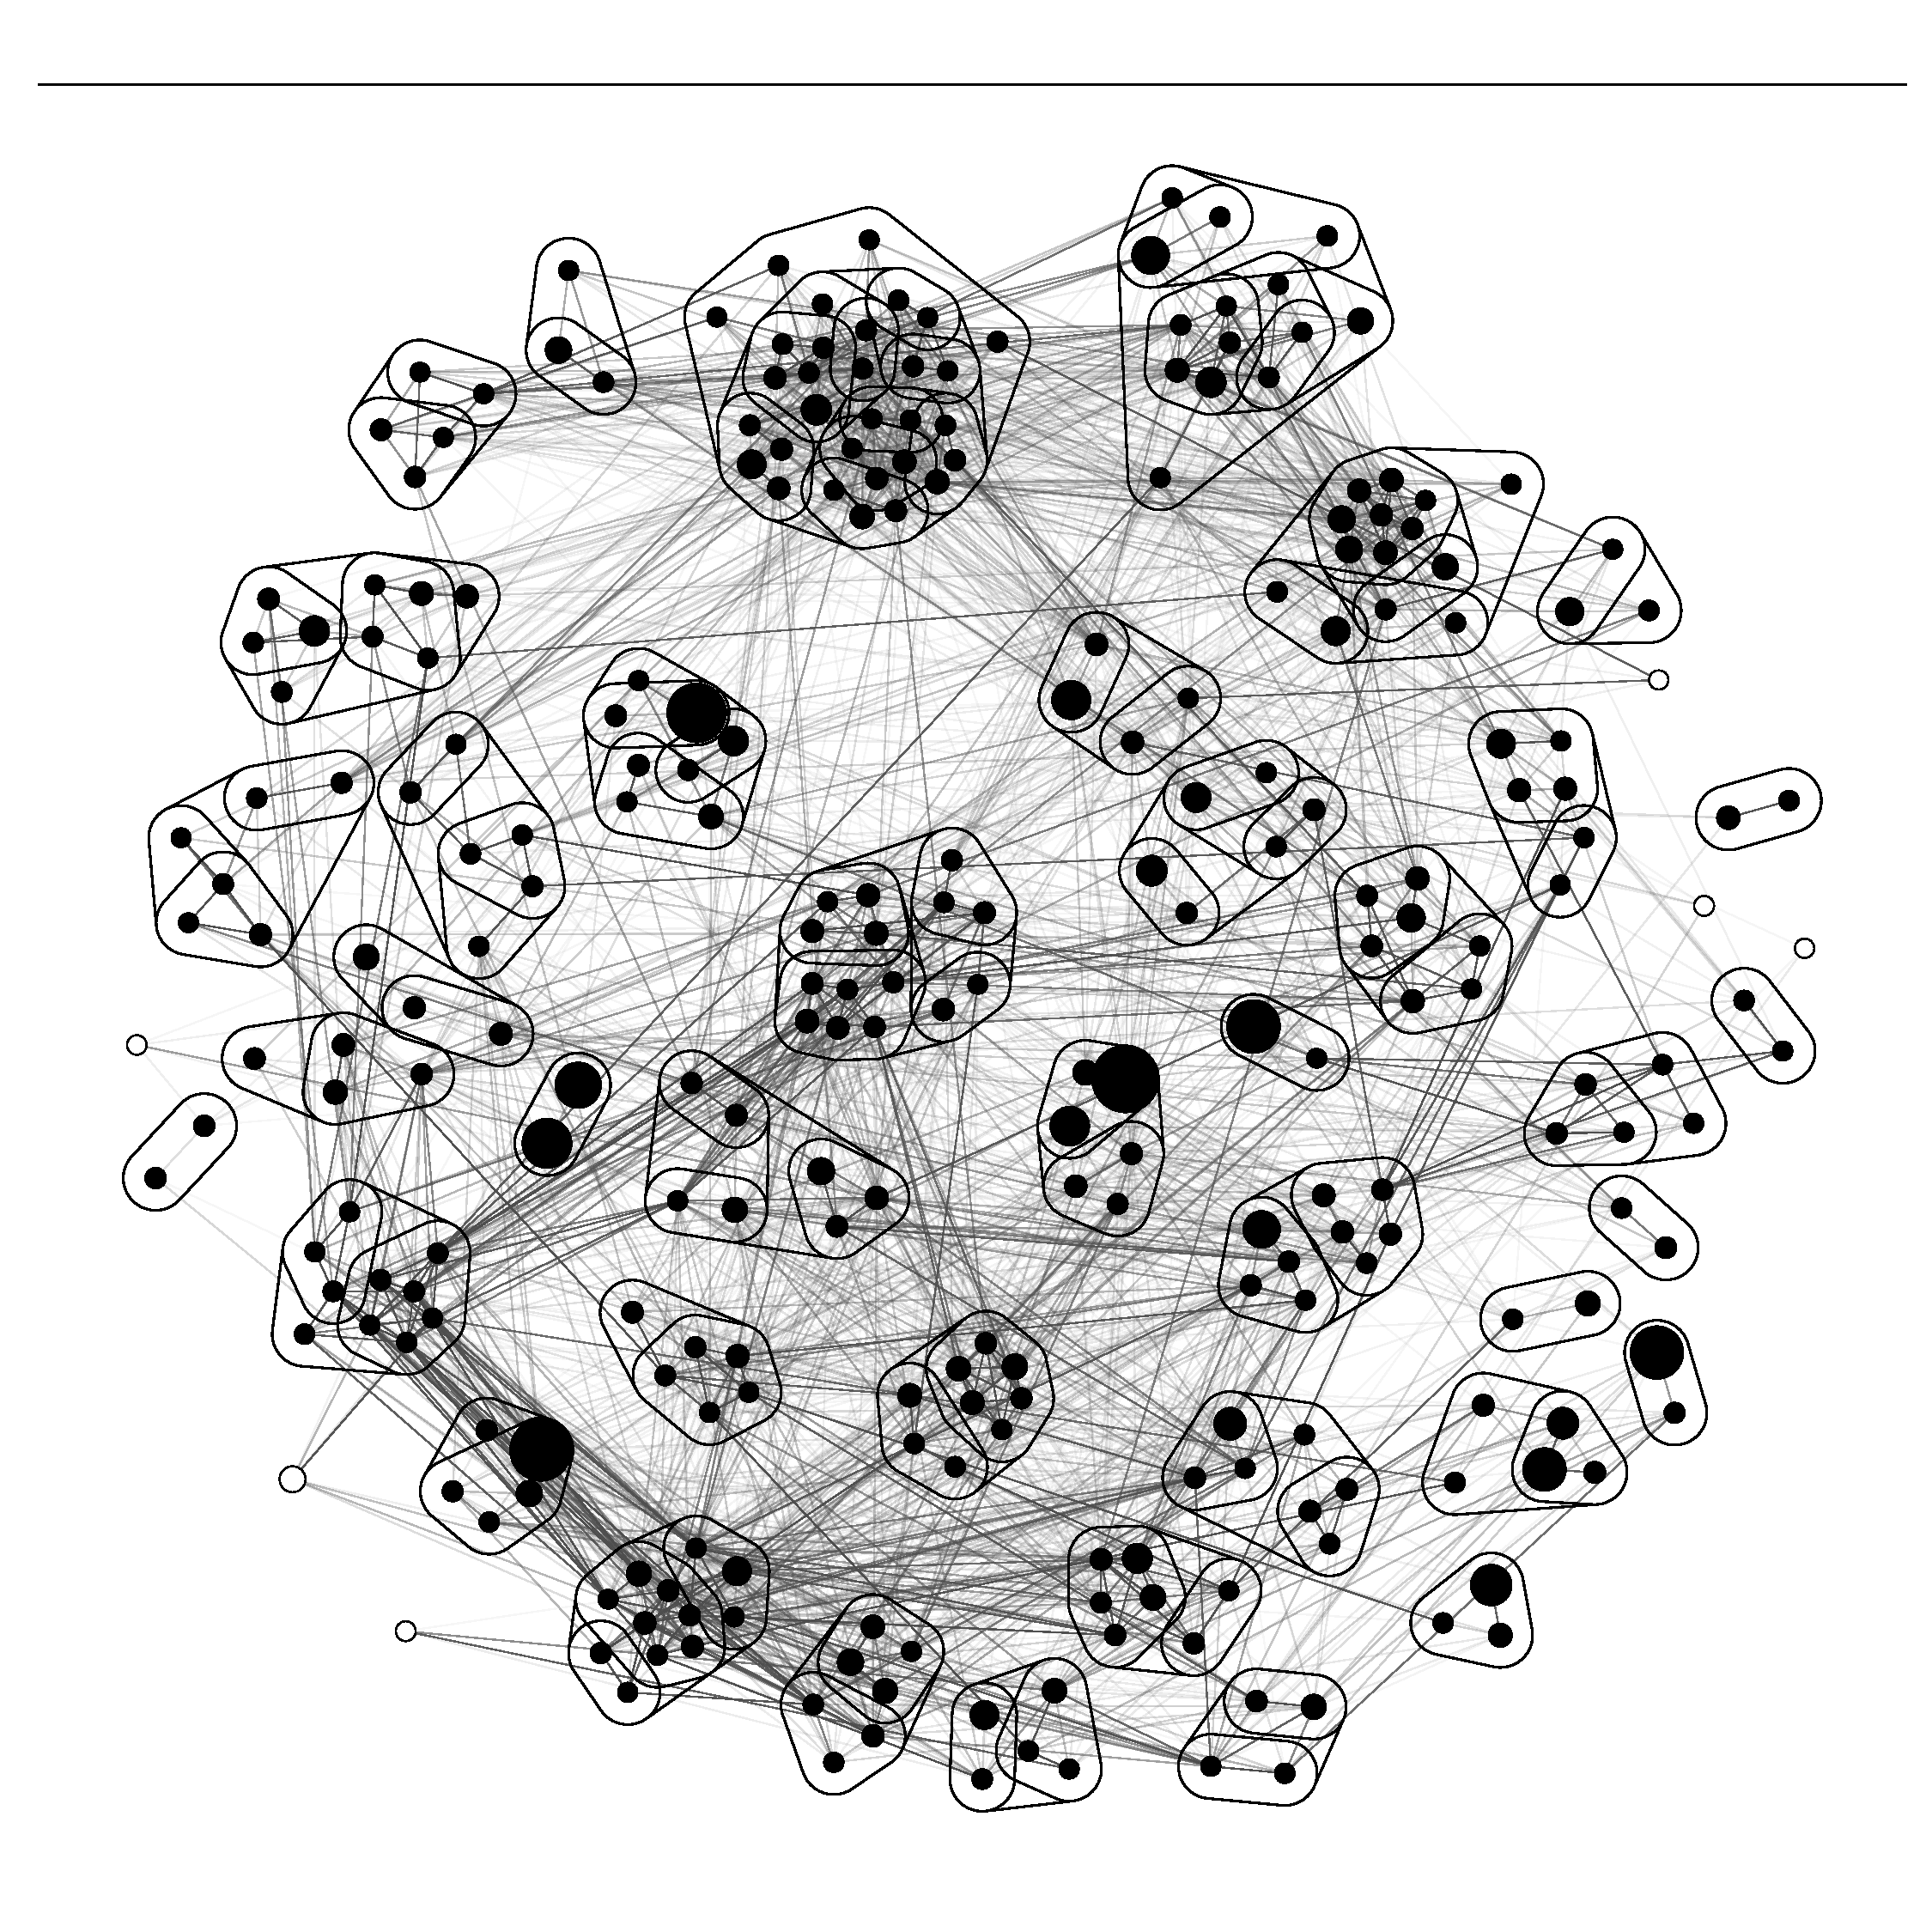
\includegraphics[width=10 cm]{fig/netvaerkskort/kort_seg_proces_niveau5_praesentation.pdf}
  \caption{}
  \label{fig_seg_proces5}
\end{centering}
\end{figure}

Klyngerne er sammensat med Moneca-algoritmen. Klyngedannelsen sker ved at aggregere erhvervsgrupperne i klynger, baseret på deres mobilitetsmønstre. Aggreringen af klynger sker ud fra beslutningsreglerne beskrevet i kapitel \ref{kap metode_sna}, hvor sammenlægningen af klynger foregår på stadigt højere niveauer - det vil sige, klynger slås sammen med andre klynger og så fremdeles - indtil der ikke længere er basis for yderligere sammenlægninger. 

Om klyngerne også er \emph{delmarkeder}, kommer i min definition an på jobmobiliteten, forstået i netværkstermer. For at der er tale om et delmarked, skal der ifølge Boje været meget mobilitet indenfor delmarkedet, og barrierer for jobmobilitet mellem  delmarkeder. Derfor bliver jobmobilitet tolket sådan, at hvis jobmobiliteten er “høj” internt i klyngerne - fra nu af kaldet \emph{den interne mobilitet} - har vi at gøre med et delmarked. 

Moneca-algoritmens klike-baserede bud på en segment-opdeling benytter jeg \emph{som udgangspunkt} for arbejdsmarkedets opdeling. Dette bud på en opdeling har jeg justeret efterfølgende, baseret på to kriterier: Et netværksanalytisk kriterie for den interne konsistens af klyngerne, baseret på to almindelige centrale mål indenfor netværksanalyse,   \emph{Densitet} og \emph{den maksimale stilængde} \parencite[68f]{Scott2000}. Et hermeneutisk kritierie, hvor noder, der forekommer malplacerede i bestemte klynger, granskes nøje for at vurdere hvor de hører til.Der er foretages nogle ganske væsentlige ændringer fra Monecas mekaniske klyngedannelsesprocedure. Dette er uddybet i bilag \ref{app_netvaerksmaal}.  

Tilsammen er jobmobilitet, \emph{densiteten} og \emph{den maksimale stilængde} for en række noder med til at sige, om vi har at gøre med et delmarked eller ej. For at parafrasere Weber, så består et delmarked af de arbejdsmarkedssituationer, hvor mobilitet er nem og typisk 
%
\footnote{Citatet lyder “\emph{A »social class« makes up the totality of those class situations within which individual and generational mobility is easy and typical.}” \parencite[302]{Weber1978}.}%
%
\parencite[302]{Weber1978}. 

Jeg vil nu gennemgå klyngedannelsen. Det er ikke kun en metodisk procedure, men tjener det formål at give en pædagogisk indføring i tolkning af det endelige netværkskort, der ellers kan fremstå temmelig uoverskueligt. 

%%%%%%%%%%%%%%%%%%%%%%%%%%%%%%%%%%%%%%%%%%%%%%
\section{Dannelsen af klynger \label{delanalyse1_segmenteringsprocessen}}
%%%%%%%%%%%%%%%%%%%%%%%%%%%%%%%%%%%%%%%%%%%%%%

Moneca-algoritmens klyngedannelse slutter på det 5. niveau. I første niveau starter vi med de 273 noder. På femte og sidste niveau er de 273 noder blevet aggreret til 41 klynger og 6 enkeltstående noder. De 6 enkeltstående noder er alle kendetegnet ved at have en meget høj intern mobilitet, og være meget specialiserede erhverv, såsom læge. 


Aggreringen fra nivea 1 til niveau 5 fremgår af tabel \ref{tab_delanalyse1_karakteristika}. Her vises ændringerne i jobmobiliteten fra niveau til niveau, som den foregår internt \emph{i} klyngerne og \emph{eksternt} mellem klyngerne.

% 
%!TEX root = ../report.tex
\begin{table}[H] \centering
\caption{Karakteristika for klyngedannelsen}
\label{tab_delanalyse1_karakteristika}
\resizebox{.8\textwidth}{!}{%
\begin{tabular}{@{}lrrrrr@{}} \toprule                         
Niveau  & 1. niveau & 2. niveau & 3. niveau & 4. niveau & 5. niveau \\    \midrule
Reduktion i antal noder & - & 137\%  & 74\% & 25\% & 13\%  \\    \midrule
Antal klynger & - & 80 & 52 & 42  & 41  \\    
Antal noder & 273 & 35 & 14  & 11  & 6  \\    
I alt ("grupper") & 273 & 115 & 66  & 53  & 47  \\    \midrule
Intern mobilitet (gns.) & 68\% & 74\% & 77\% & 79\% & 81\% \\    
Ekstern mobilitet (gns.)  & 32\% & 26\% & 23\% & 21\% & 19\% \\    
Mobilitet i alt & 100\%  & 100\%  & 100\%  & 100\%  & 100\%  \\    \midrule
Forøgelse i intern mobilitet i procent  & - & 9\% & 3\%  & 2\%  & 3\%  \\    
Forøgelse i intern mobilitet i procentpoint & - & 6\%  & 2\%  & 2\%  & 3\%  \\    
\end{tabular} }
\end{table}



% 

Det første iøjnefaldende er at den interne mobilitet på det (uaggregerede) niveau 1 er højt i sig selv: 68 \%. Det indikerer at en væsentlig mængde skift foregår på et meget detaljeret \texttt{DISCO}-niveau. Langt de fleste bliver indenfor deres eget job%
%

\footnote{Eller ihvertfald et job, der ligger så tæt på, at man selv på mit usædvanligt lave 4-cifrede \texttt{ISCO}-niveau ikke kan skelne dem fra hinanden.}%
%
. Det understøtter i høj grad Gruskys antagelse om, at blah blah læs det han skriver om mikroklasser \#todo). 

Fra niveau 1 til niveau 2 er Moneca er i stand til at forhøje den interne mobilitet med 6 procentpoint, således at næsten $\nicefrac{3}{4}$ af jobmobiliteten foregår indenfor klyngerne. Niveau to klynger på meget lavt niveau, og kunne på en måde siges at være en slags “udvidede erhvervsgrupper,” med gennemsnitligt antal noder i klyngerne på 3,5%
%
\footnote{ 3,2 hvis man tæller de 36 noder med, der endnu ikke er aggregerede.}%
%


Der er, så vidt jeg ved, ikke tidligere foretaget en jobmobilitetsundersøgelse på så detaljeret et Disco-niveau og med så omfangsrigt et datamateriale i Danmark. Men vi kan konstatere, at det er i overenstemmigelse med tidligere undersøgelser, der viser at hovedparten af skift i job sker indenfor relativt afgrænsede delmarkeder \parencite[124]{BojeToft1989}. 

Det danske arbejdsmarked må siges at være voldsomt specialiseret, blot ved at se på de første to Moneca-niveauer. 

Jeg vil nu gennemgå udviklingen i niveauerne visuelt, og beskrive udviklingen ud fra tabel \ref{tab_delanalyse1_karakteristika}.

Figurerne der afbilleder processen skal tolkes således: Der er hvide og sorte noder tegnet ind på netværkskortene på side \pageref{fig_delanalyse1_kort_seg_proces2} til side \pageref{fig_delanalyse1_kort_seg_proces5} . Forskellen på hvide og sort noder i figurerne på er simpel: Sorte node indikerer at denne node er blevet inkluderet i en ny klynge siden det foregående niveau. Hvid node indikerer at den \emph{ikke} er blevet inkluderet i en ny klynge siden niveauet før. 
Niveau 1 er ikke afbilledet, da der ikke findes et foregående niveau at vise et skift fra. 
Forbindelserne mellem noderne er markeret med grå streger, men bør ikke tolkes på nuværende tidspunkt, da der ikke er diffentieret mellem stærke og svage forbindelser i illustrationerne. 


%%%%%%%%%%%%%%%%%%%%%%%%%%%%%%%%%%%%%%%%%%%%%%
\newpage \subsection{Niveau 2}
%%%%%%%%%%%%%%%%%%%%%%%%%%%%%%%%%%%%%%%%%%%%%%


\begin{wrapfigure}{r}{8cm}
  \vspace{-20pt}
  \begin{center}
   \caption{}
   \label{fig_delanalyse1_kort_seg_proces2}
    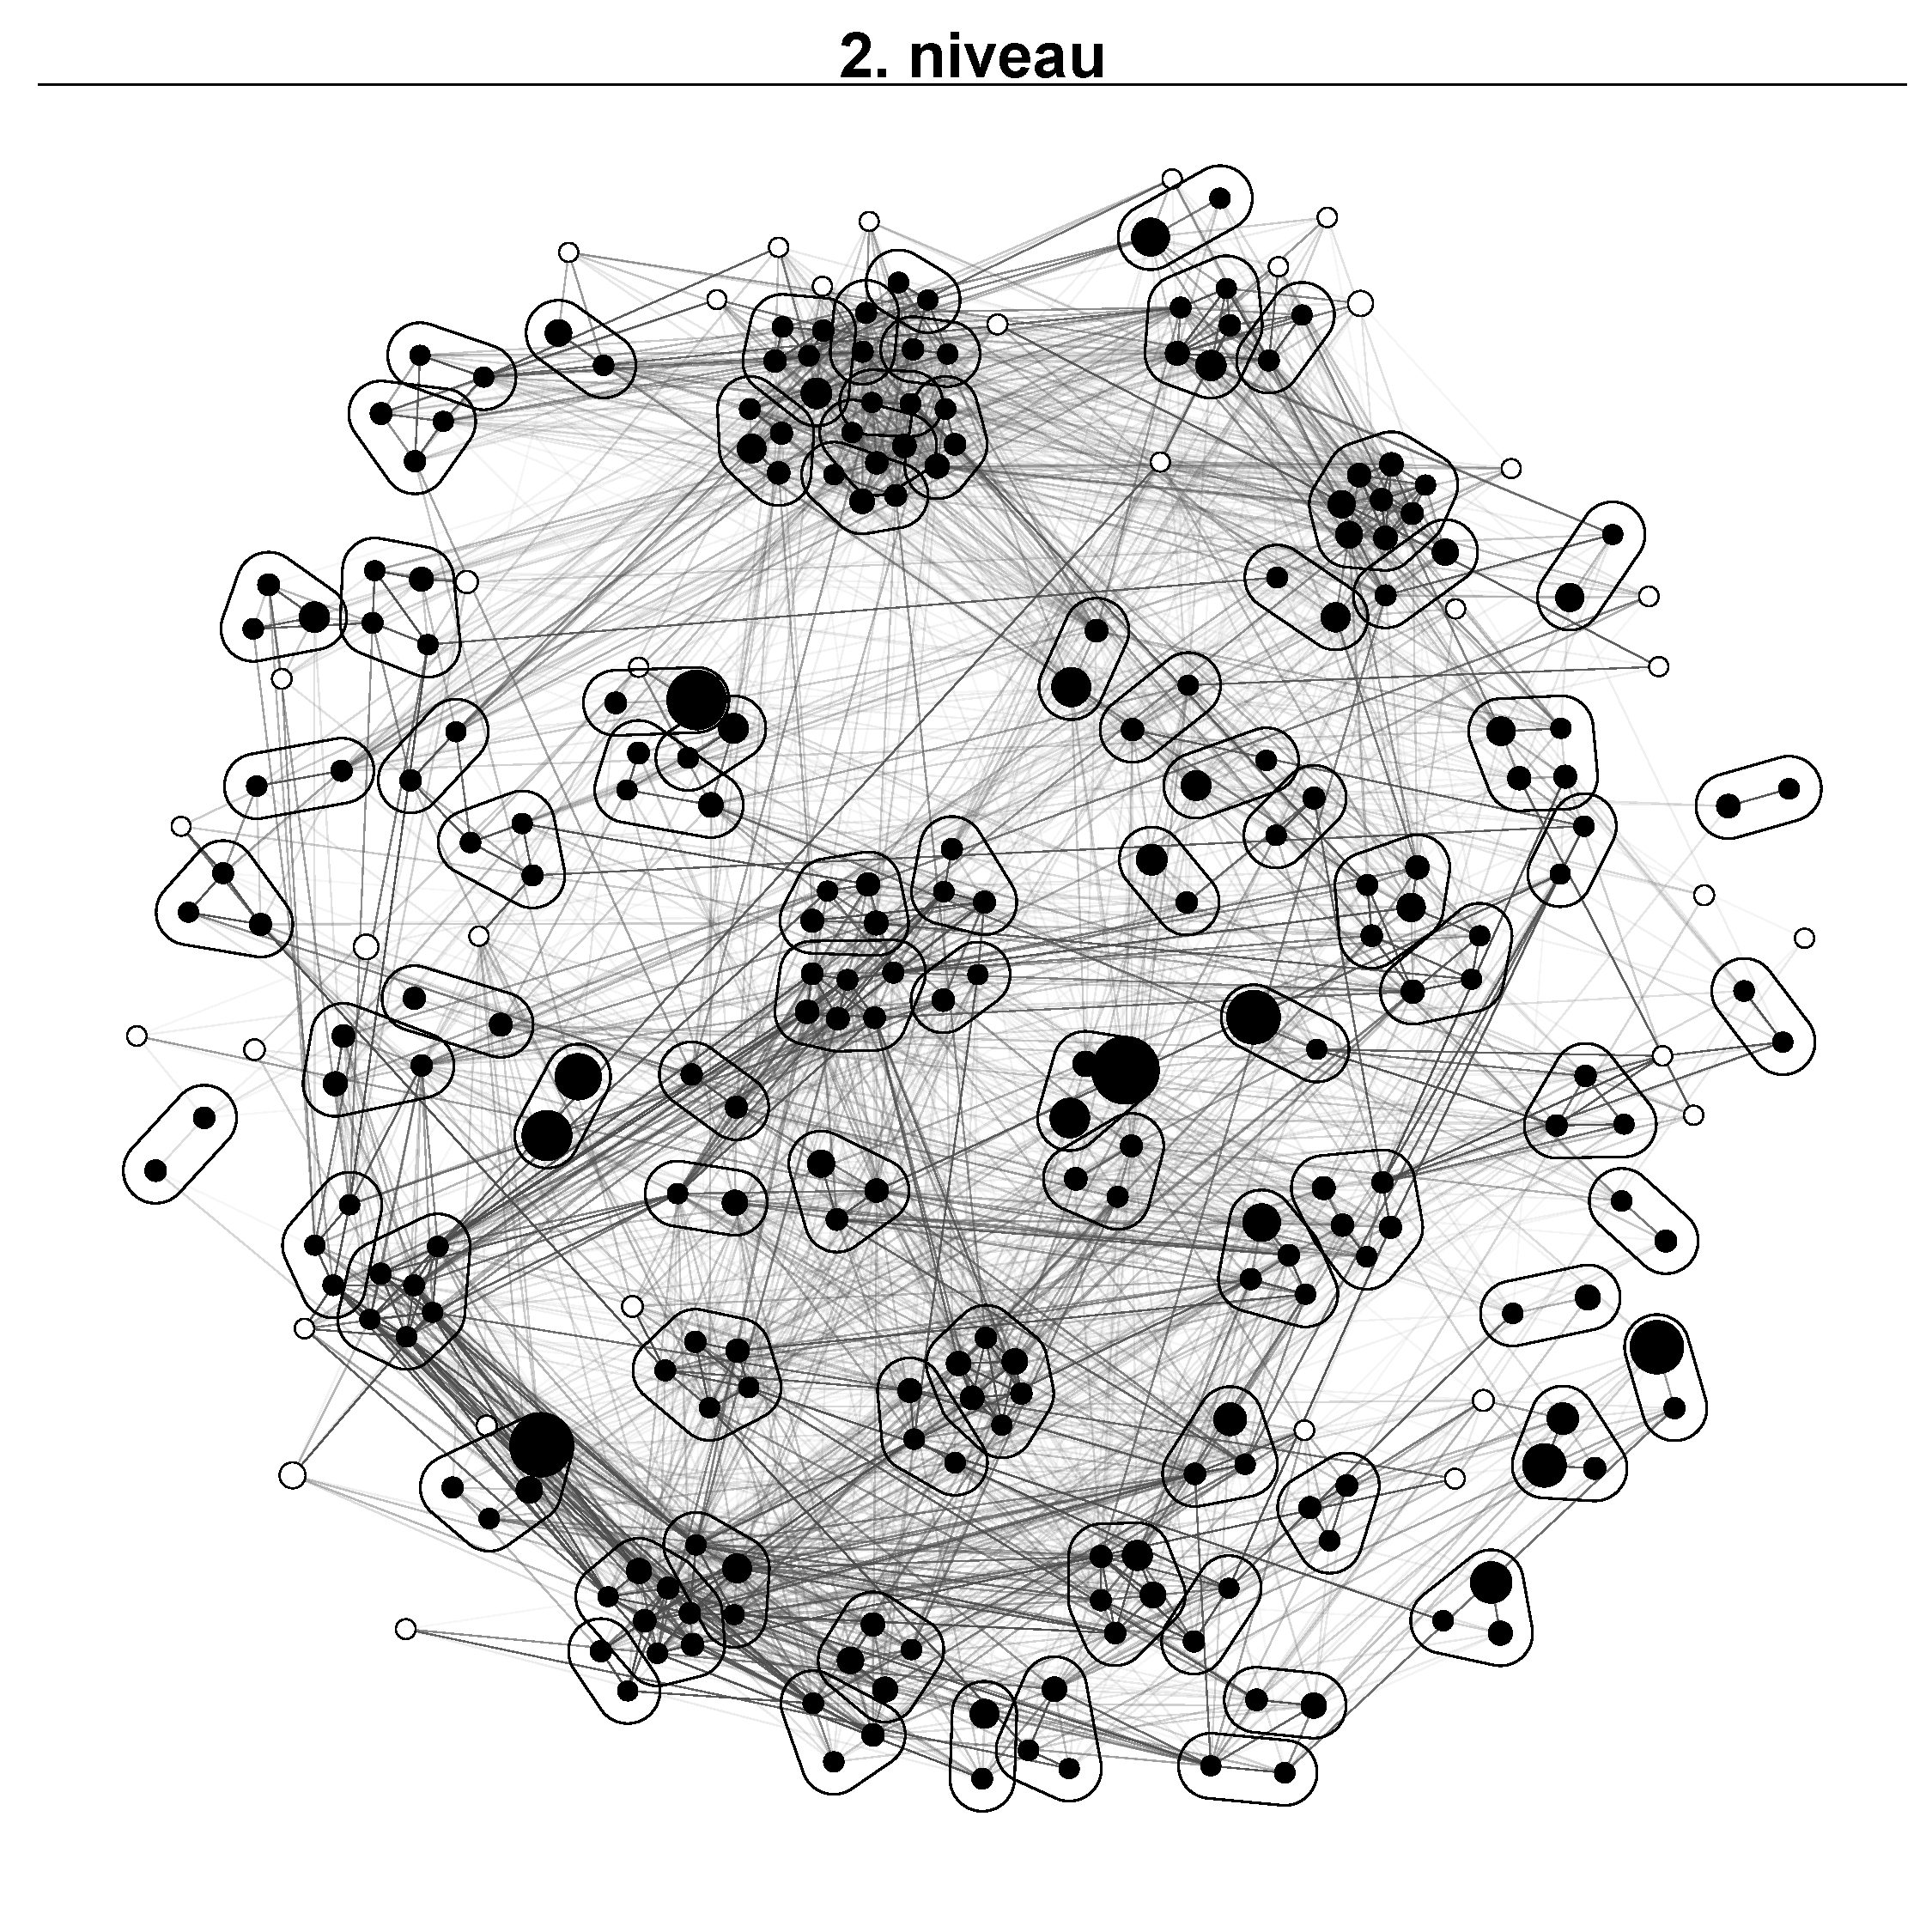
\includegraphics[width=8cm]{fig/netvaerkskort/kort_seg_proces2.pdf}
    \label{fig_delanalyse1_kort_seg_proces2}
  \end{center}
  \vspace{-20pt}
\end{wrapfigure}

Den mest markante aggregering i klynger og stigning i intern jobmobilitet fra finder sted i skiftet fra 1. niveau til 2. niveau, og herefter falder effekten af klyngedannelsen på den interne jobmobilitet støt. Af figur \ref{fig_delanalyse1_kort_seg_proces2} fremgår aggreringen. 

På 2. niveau går vi fra de oprindelige 273 fritstående noder til 80 klynger, samt 35 endnu fritstående noder: 115 i alt%
%
\footnote{ Der skelnes i tabel \ref{tab_delanalyse1_karakteristika} ikke mellem enkelte noder og klynger, da klyngernes interne mobilitet jo netop skal erstatte nodernes, og en direkte sammenligning derfor er ønskelig.}%
%
. Antallet af klynger er reduceret med 137 \%, og den gennemsnitlige interne mobilitet i klyngerne er steget med 6 procentpoint. 


%%%%%%%%%%%%%%%%%%%%%%%%%%%%%%%%%%%%%%%%%%%%%%
\newpage \subsection{Niveau 3}
%%%%%%%%%%%%%%%%%%%%%%%%%%%%%%%%%%%%%%%%%%%%%%

\begin{wrapfigure}{r}{8cm}
  \vspace{-20pt}
  \begin{center}
   \caption{}
   \label{fig_delanalyse1_kort_seg_proces3}
    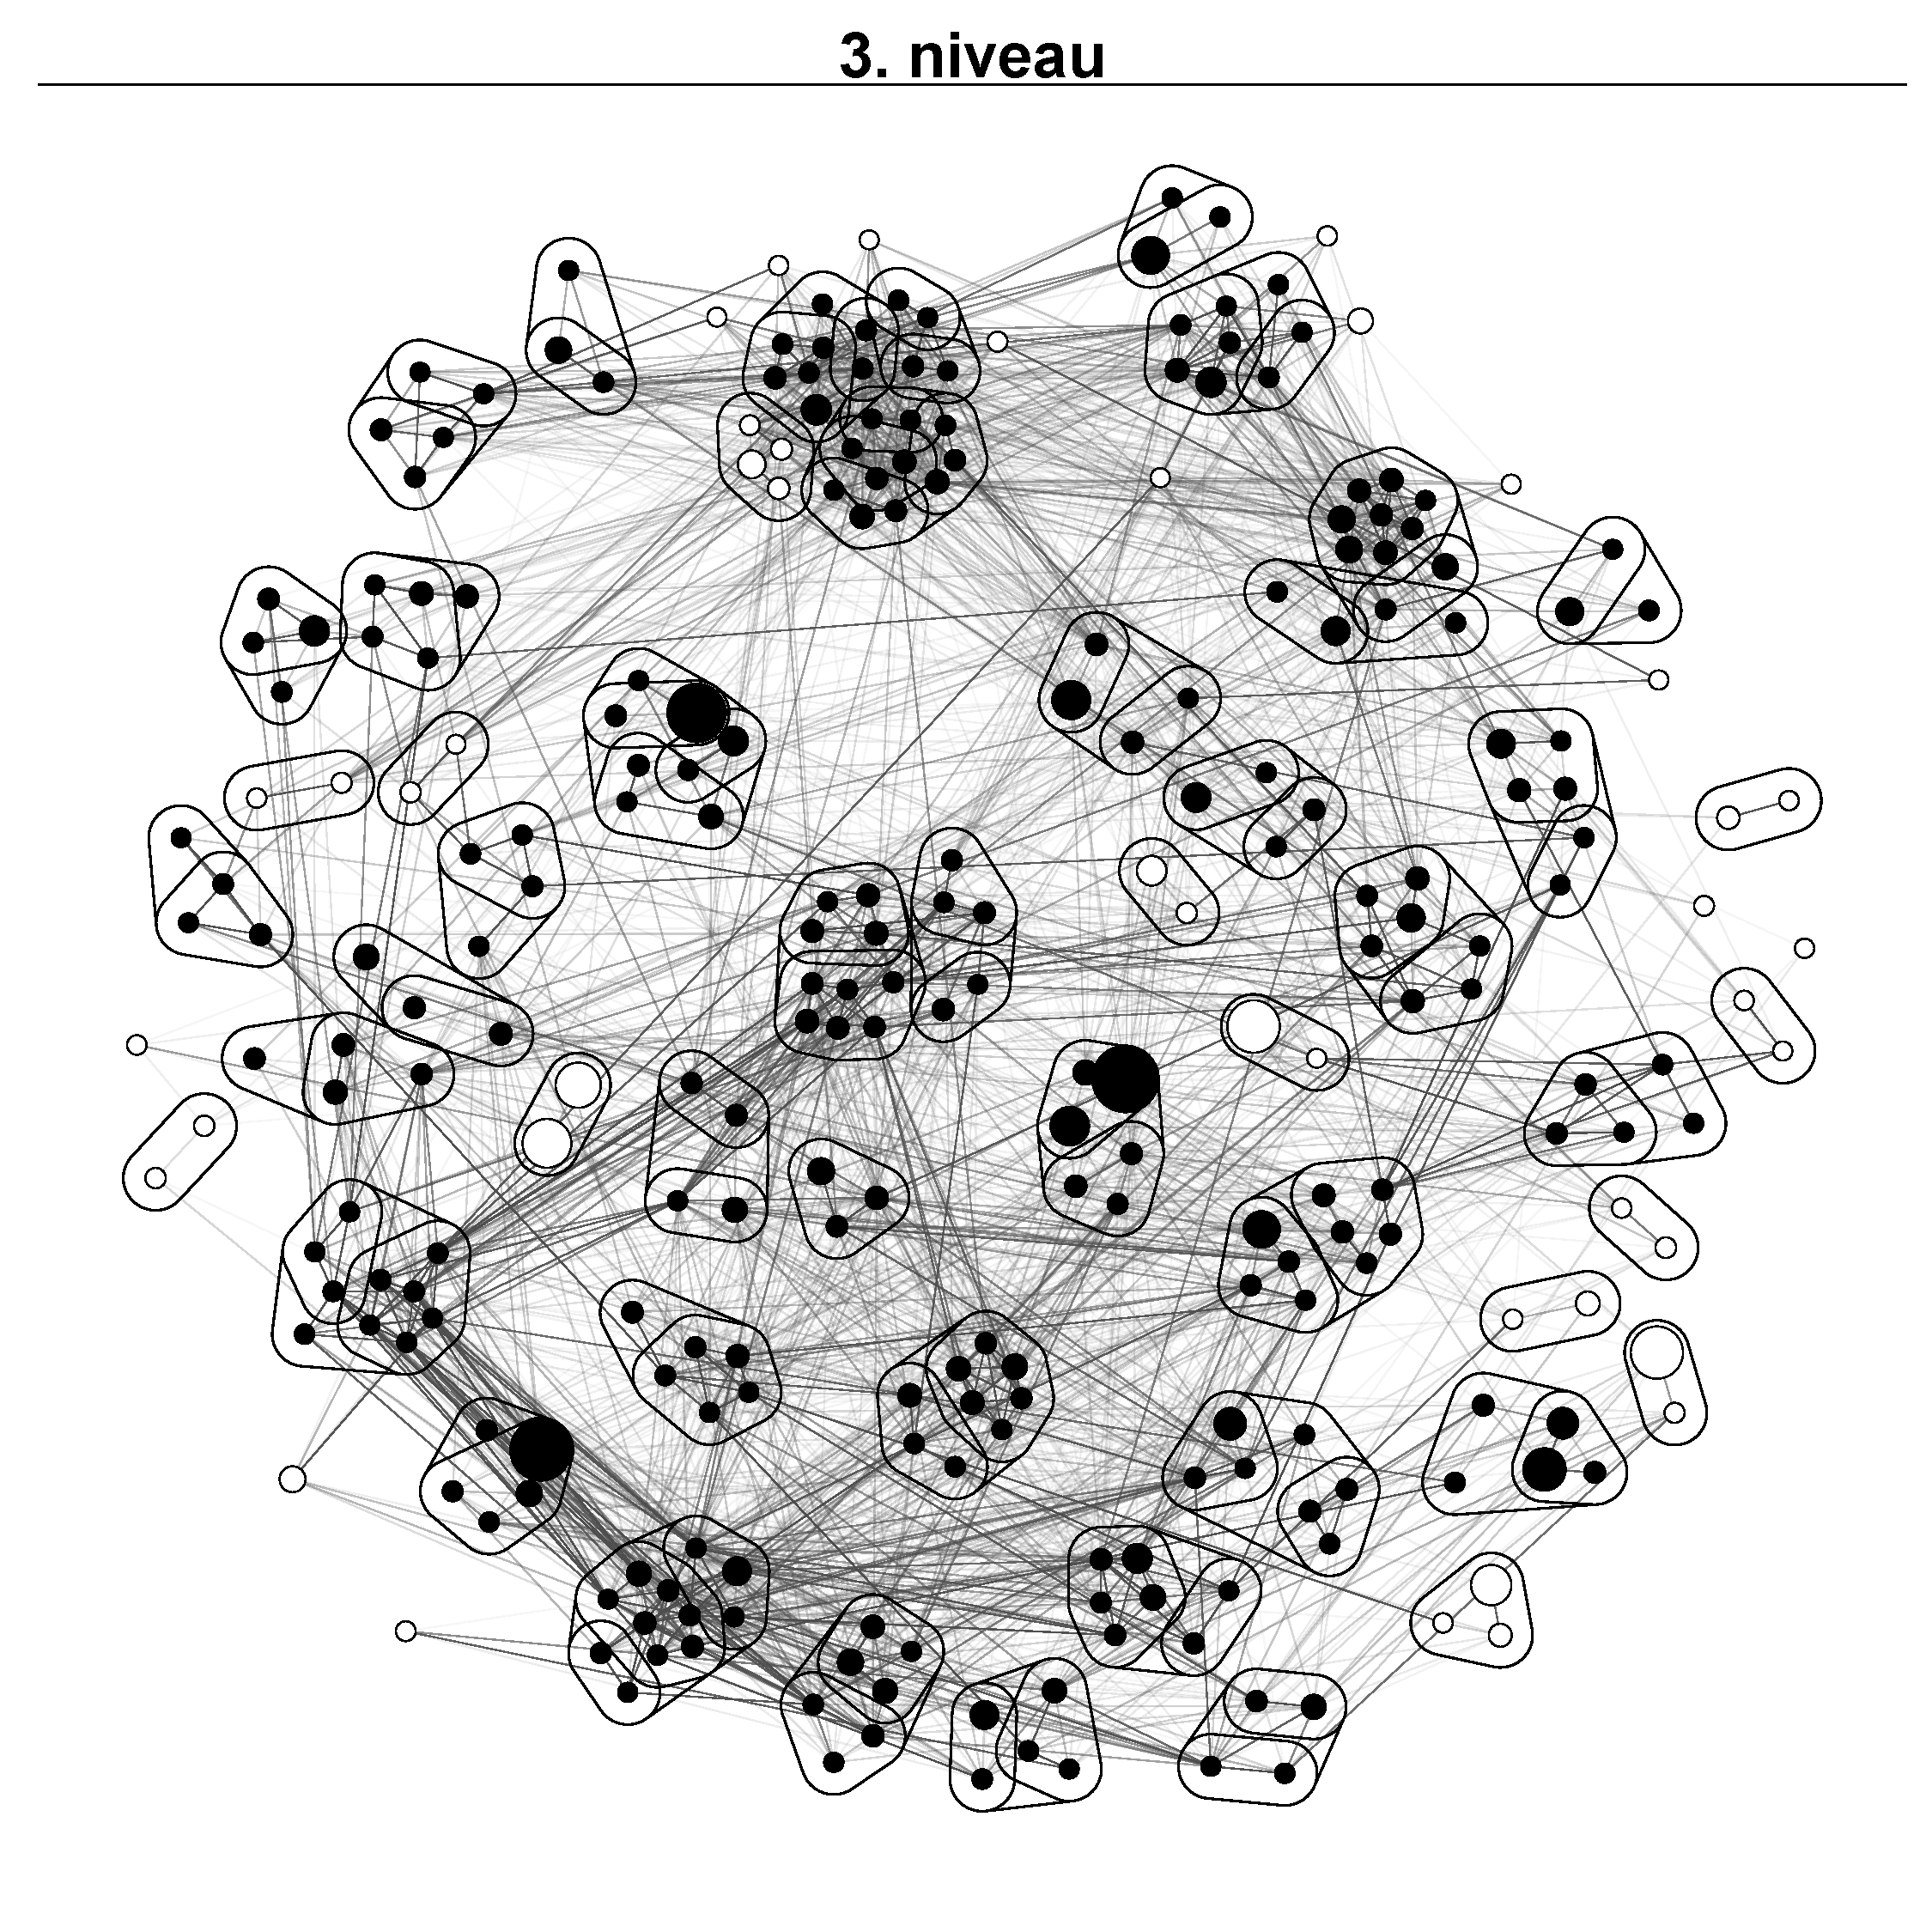
\includegraphics[width=8cm]{fig/netvaerkskort/kort_seg_proces3.pdf}
    \label{fig_delanalyse1_kort_seg_proces3}
  \end{center}
  \vspace{-20pt}
\end{wrapfigure}

På 3. niveau, afbilledet i figur \ref{fig_delanalyse1_kort_seg_proces3}, inkluderes 21 enkeltstående noder i klynger, samt en række niveau 2 klynger aggrereres yderligere. Det reducerer antallet af klynger til 52 og 14 enkeltstående noder, 66 grupper i alt. Stigningen i den gennemsnitlige interne mobilitet er på 2 procentpoint, hvilket er beskedent sammenlignet med stigningen fra niveau 1 til niveau 2. Tilgengæld er reduktionen i \emph{antallet} af grupper på 74\%. Det vil sige at kompleksiteten i netværket reduceres, samtidig med at den interne mobilitet øges. Det er tendensen fra niveau 3 og frem: Der foretages stadig væsentlige sammenlægninger af klynger og noder til større klynger, men betydning af sammenlægningen på den gennemsnitlige interne mobilitet forbliver derefter på de to-tre point per niveau. Det ender dog alligevel med at blive en forøgelse i alt på 7 procentpoint, altså omtrent det samme som forøgelsen fra niveau 1 til niveau 2. 

% Det tolker jeg som udtryk for, at jo længere væk fra den sociale kontekst af den oprindelige erhvervsgruppe, vi kommer, desto mindre systematik er der i jobskiftet: Det bliver sværere at pege på de meget


%%%%%%%%%%%%%%%%%%%%%%%%%%%%%%%%%%%%%%%%%%%%%%
\newpage \subsection{Niveau 4}
%%%%%%%%%%%%%%%%%%%%%%%%%%%%%%%%%%%%%%%%%%%%%%

\begin{wrapfigure}{r}{8cm}
  \vspace{-20pt}
  \begin{center}
   \caption{}
   \label{fig_delanalyse1_kort_seg_proces4}
    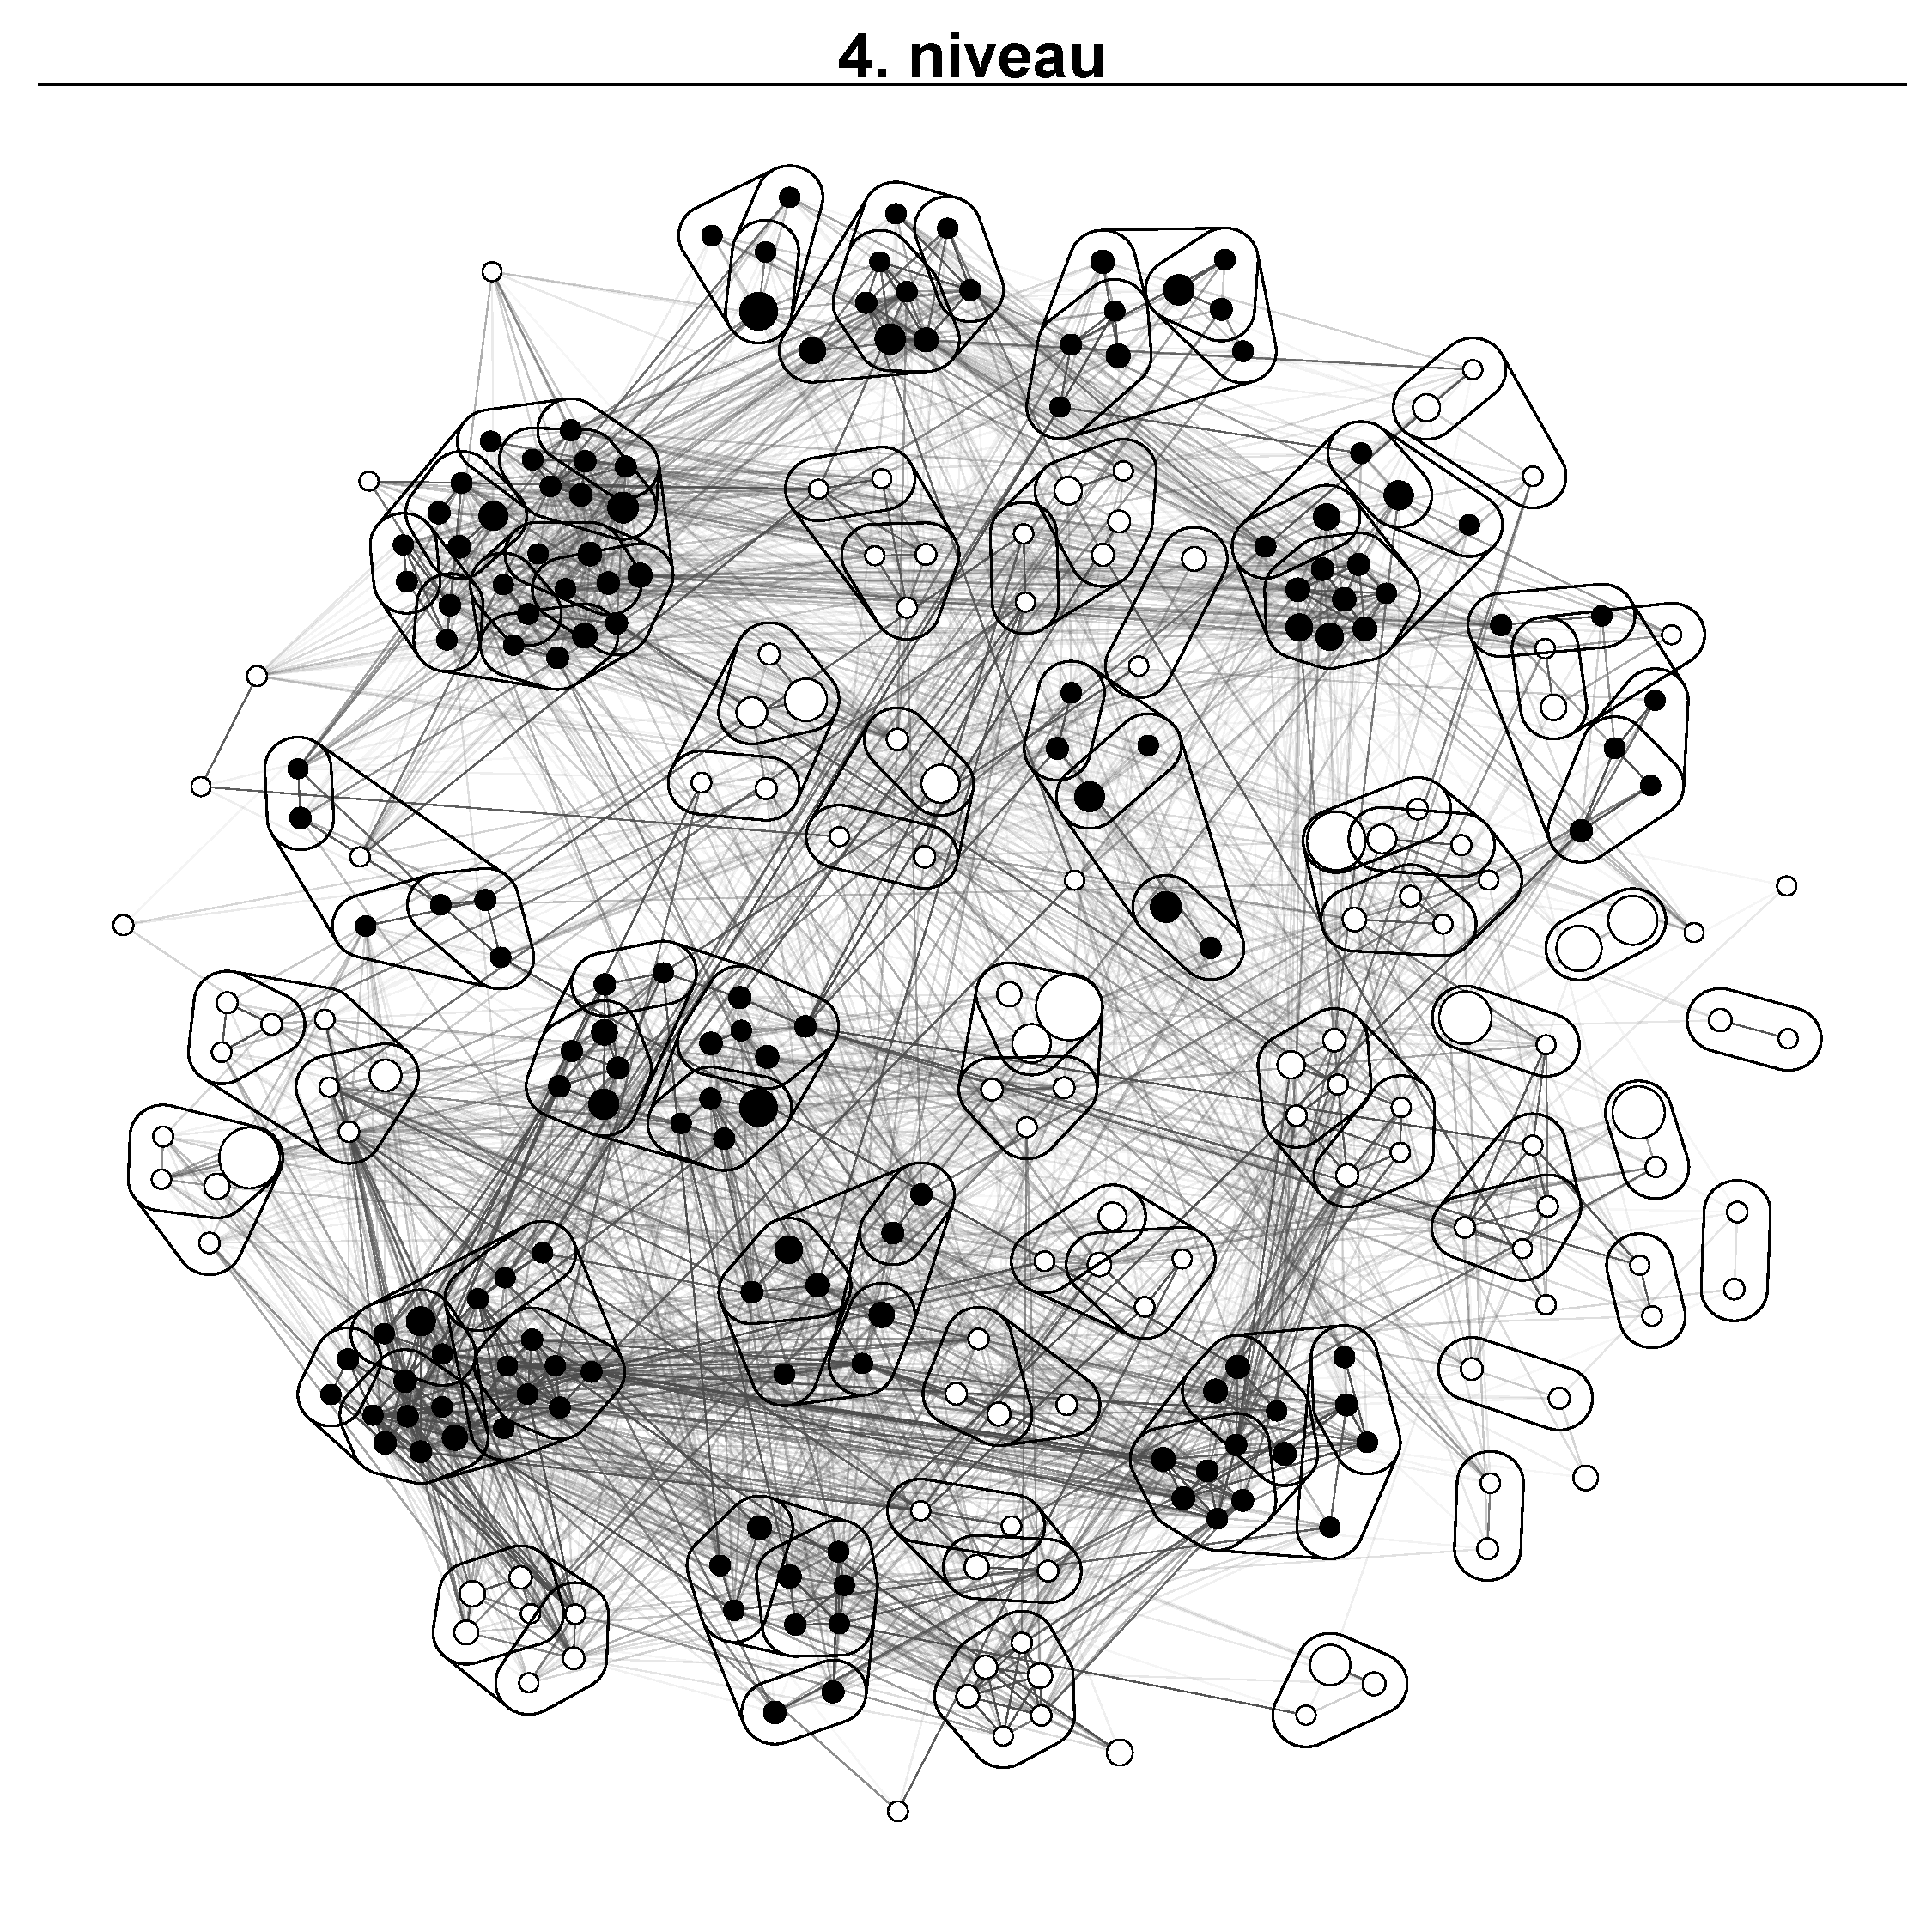
\includegraphics[width=8cm]{fig/netvaerkskort/kort_seg_proces4.pdf}
  \end{center}
  \label{fig_delanalyse1_kort_seg_proces4}
  \vspace{-20pt}
\end{wrapfigure}

På 4. niveau skabes 10 nye klynger. Der er nu 53 grupper, hvoraf 42 er klynger og 9 er noder. Den interne mobilitet er igen steget med to procentpoint. Dette kan måske forekomme beskedent, men jeg vil faktisk mene det forholder sig omvendt: At kunne forklare yderligere to procent af den samlede variation i jobskifte, er mere end udemærket. Især når reduktionen i antallet af grupper er på $\nicefrac{1}{4}$. 


Det er på dette niveau, at sammenlægningerne binder allerede store klynger sammen, og vi får udvidede klynger med en betragtelig mængde forskellige erhvervsgrupper samlet under ét. Det er altså her, det for alvor bliver interessant. 
Disse klynger af erhvervsgrupper nemlig ikke er ikke baseret på den \emph{teknisistiske vision}, som Grusky advarer imod, og heller ikke en a priori teoretisk opdeling, som hos Goldthorpe og Oesch. Inddelingen er istedet baseret på den sociale nærhed, der antages at findes mellem jobs, hvor mobilitet er “let og typisk” , som Weber siger er det definerende træk ved social klasse. Jeg er dog som tidligere beskrevet mere beskeden, og prøver kun at udtale mig om økonomiske klasser- og klassefraktioner.  %kalder det, sin beskrivelse af (et af) de definerende træk ved social klasse: Individuel mobilitet% Det her skal nok stå i teori-afsnittet, og så henvises til her i stedet. \#todo

%
\footnote{Der er naturligvis flere elementer end individuel jobmobilitet på spil. Det fulde citat lyder: “\textit{A »social class« makes up the totality of those class situations within which individual and generational mobility is easy and typical.}” \parencite[302]{Weber1978}. }% Det her citat står allerede længere oppe. Lav vurdering af hvor det hører til senere. 
%

%%%%%%%%%%%%%%%%%%%%%%%%%%%%%%%%%%%%%%%%%%%%%%
\newpage \subsection{Niveau 5 \label{delanalyse1_endelige mobilitetskort}}
%%%%%%%%%%%%%%%%%%%%%%%%%%%%%%%%%%%%%%%%%%%%%%

Det 5. niveau er det sidste niveau, da Moneca-algoritmen ikke kan aggregere klynger på et højere niveau end det. Vi mindes fra gennemgangen af Moneca-proceduren på side  \pageref{metode_monecastepbystep}, at det betyder, at Moneca ikke kan finde nogle noder eller tidligere klynger, hvor der er intern mobilitet mellem  \emph{alle} klynger fra niveauet tidligere. %check lige op på det med Anton \#todo 
I skiftet fra niveau 4 til 5 aggregeres to klynger. Den ene skabes ud fra store niveau 4-klynger, og inkluderer en enkelt node i processen, \emak{d8110}. Den anden er én stor niveau 4-klynge, der “sluger” 4 enkeltstående noder. 

Det bringer os ned på de 41 klynger og 6 noder.



\begin{figure}[H]
\begin{centering}
  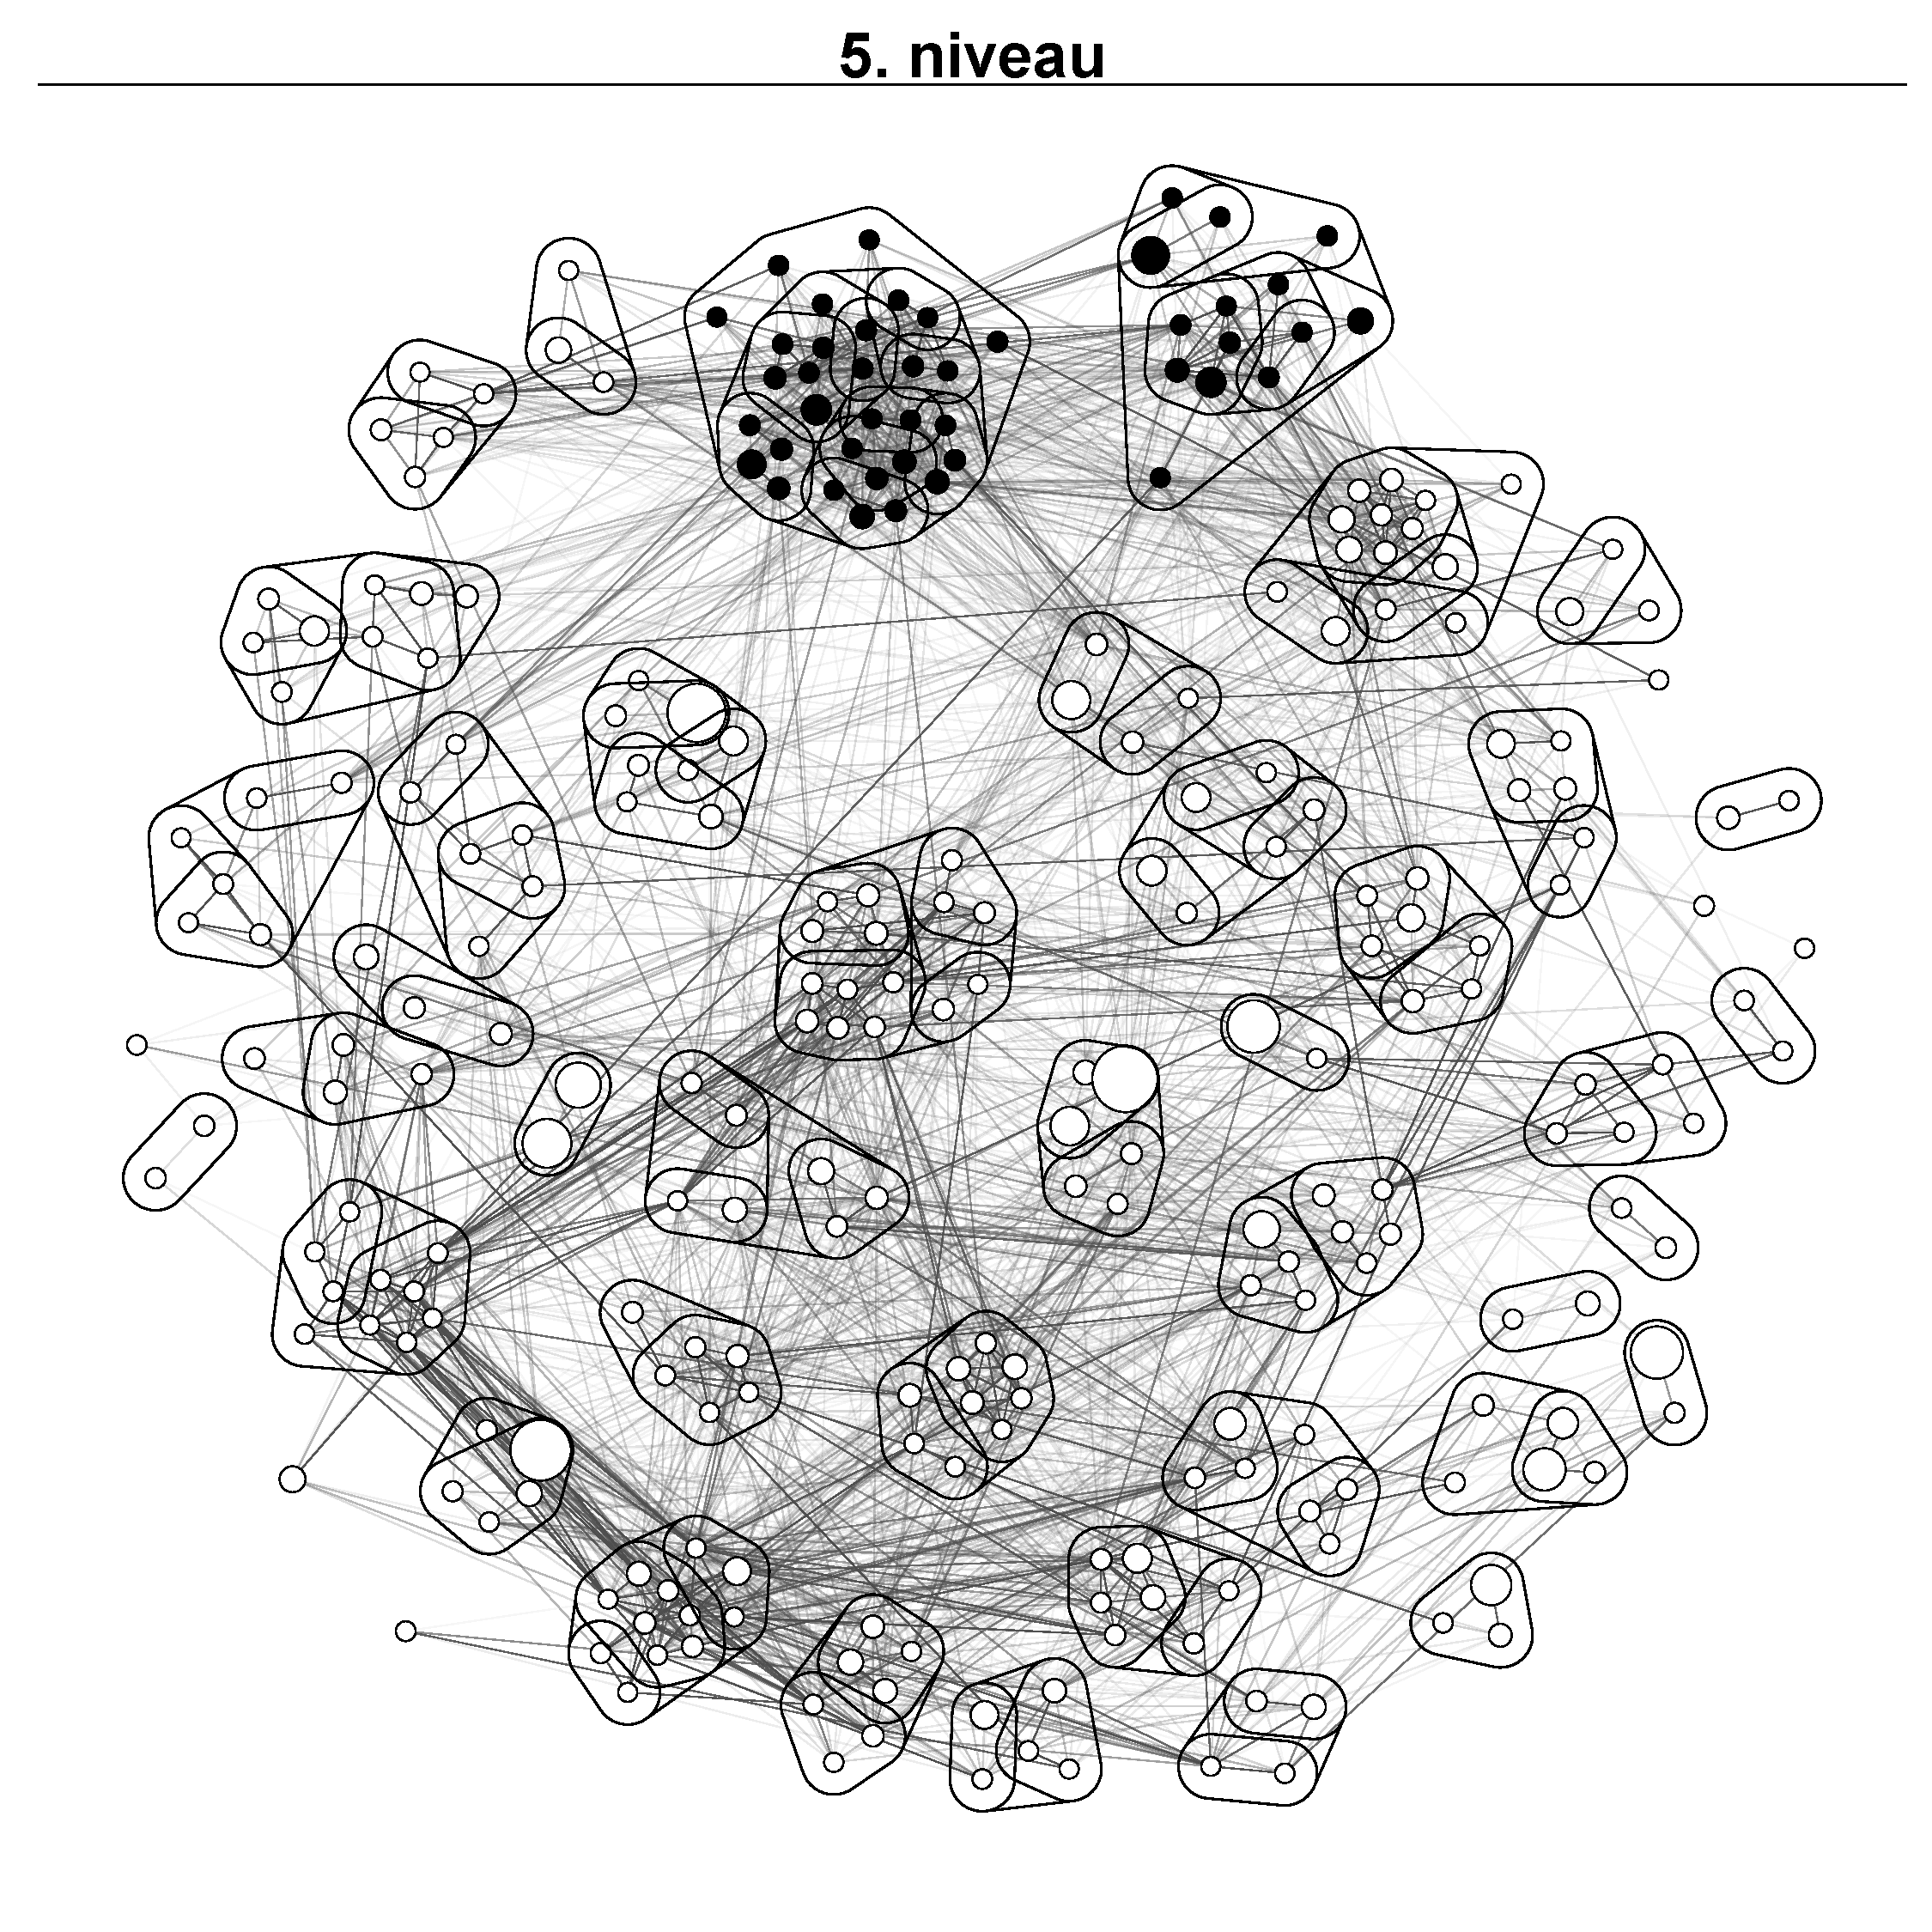
\includegraphics[width=10 cm]{fig/netvaerkskort/kort_seg_proces5.pdf}
  \label{fig_delanalyse1_kort_seg_proces5}
  \caption{}
\end{centering}
\end{figure}







Den oprindelige 273 x 273 mobilitetstabel nu er reduceret til en mere overkommelig 47 x 47 mobilitetstabel. Tabel \ref{tab_delanalyse1_noegletalniveau1og5} viser yderligere centrale mål for startniveau 1 og slutniveau 5. Disse viser tydeligt at aggregeringen har skabt færre kategorier med højere intern mobilitet. 

Vi ender med en gennemsnitlig intern mobilitet på 81 \% Dette forekommer rimeligt og acceptabelt, og en stigning på 13 procentpoint i den interne mobilitet fra niveau 1 til niveau 5 vurderer jeg som meget tilfredsstillende. Det endelige resultat forklarer omtrent $\nicefrac{4}{5}$ af al mobilitet på arbejdsmarkedet, selvom det er vigtigt at huske på den meget høje interne mobilitet, der forekommer indenfor erhvervsgrupperne på det danske arbejdsmarked. 



%
%!TEX encoding = UTF-8 Unicode
%!TEX root = ../report.tex
% Table generated by Excel2LaTeX from sheet 'delanalyse1_noegletalniveau1og5'
\begin{table}[htbp]
  \centering
  \caption[Nøgletal for første og sidste niveau i klyngedannelsen]{Nøgletal for (det uaggregerede) niveau 1 og (det endelige) niveau 5}
  \resizebox{.8\textwidth}{!}{%
    \begin{tabular}{lcccccc}
          &       & gns. intern & sd afvigelse  &       &       &  \\
    Niveau & grupper &  mobilitet & 
\emph{\tiny{(i procentpoint)}} & median & min   & max \\
    \midrule
    1. niveau & 273   & 68\%  & 12    & 68\%  & 43\%  & 97\% \\
    5. niveau & 47    & 81\%  & 10    & 80\%  & 54\%  & 96\% \\
    \bottomrule
    \end{tabular}}%
  \label{tab_delanalyse1_noegletalniveau1og5}%
\end{table}%

%

gennemsnittet på det 1. niveau er på 68 \%, mens det på 5. niveau er steget til 80 \%. Medianen har så godt som ens værdier. Standardafvigelsen for den interne mobilitet på det 1. niveau er på 12 \%, mens den på det 5. niveau er på 10 \%. At standardafvigelsen er faldet, mens gennemsnittet er steget, er vigtigt, fordi det fortæller os, at gennemsnittet ikke er trukket op via enkelte klynger. Det understøttes af medianens værdi, der er meget tæt på gennemsnittet. Alle tre forhold viser os, at det en \emph{generel} og \emph{stabil} forbedring af mobilitetsstrukturen: På de tre mest fundamentale centralitetsmål for kontinuerte variable er der sket en forbedring \parencite[121]{Malchow-MoellerWuertz2010}. Det ses også ud fra minimumsværdierne. Hvor de laveste værdier tidligere lå på lidt over 40 \%, ligger de nu på lidt over 50 \%.


Konklusionen er, at 5. niveau forklarer \emph{mere} mobilitet, og den den gennemsnitlige mobilitet varier gennemsnitligt \emph{mindre} end i noderne på 1. niveau. Et højere aggregeringsniveau ud fra Monecas beslutningsprocedure forklarer følgelig \emph{hvor} mobiliteten løber hen, når den bevæger sig udenfor de oprindelige erhvervsgrupper: Når folk søger andet arbejde end indenfor deres erhvervsgruppe, kan netværksmodellen forklare 13 \% mere af mobiliteten end den oprindelige mobilitetstabel. Det kan også ses på følgende måde: Af de 32 \% af mobiliteten, der ikke foregår internt i erhvervsgrupperne, kan netværksmodellen forklare 41 \% af den eksterne jobmobilitet%
%
\footnote{ Det kunne være særdeles interessant at sammenligne med en latent klasseanalytisk-, klyngeanalytisk- eller faktoranalytisk tilgang. Det er desværre for omfattende for dette speciale, med dets ambition om at benytte Monecas netværksanalytiske metode i dybden.}
%


% Det er jo sådan set også det, den er designet til, kunne man indvende. Men det tilfredsstillende her er at helt op til \emph{det 5. aggregreringsniveau} er der stadig en bedre forklaringskraft end på de tidligere niveauer. Man kunne forestille sig at for mange kompromisser med sammenlægninger - genkald argumentet fra side ??(det om at der lægger noder sammen der rent faktisk ikke hænger sammen \#todo) ville fungere kontraproduktivt over et vist niveau, men det er altså ikke tilfældet. % ved ikke helt om det her argument egentligt holder -vil en større sammenlægning ikke bare automatisk give bedre forklaring? Nej! for hvis en node nu har meget mere udveksling med en node udenfor det, den er lagt sammen med, så ville det jo godt kunne trække ned. Men det sker ikke her, altså er det en god sammenlægning. Tror jeg. 

Et vigtigt forhold er, at visse klynger indeholder langt flere beskæftigede end andre, og kan derfor anses som sammenlægninger, der er mere væsentlige end andre. Vi får dermed nogle klynger, der antalsmæssigt beskæftiger store dele af den danske befolkning. Dette vil jeg mene er et andet vigtigt parameter i klyngedannelsen, så længe at det ikke bryder med kravet om delmarkedsstatus, hvilket min gennemgang viser at det ikke gør: 


I dette afsnit er aggreringen fra niveau til niveau blevet beskrevet med henblik på at vurdere om vi kan tale om delmarkeder fremfor blot klynger. Selv med en mere grov opdeling end Monecas klike-baseredede inddeling står det klart, at det danske arbejdsmarked som minimum udgøres af mere end 3 delmarkeder.  Der er en langt mere fraktioneret struktur i det danske arbejdsmarked, hvilket også teoretisk er blevet forudsagt (find eksempel fra Boje \#todo). 


Et af nøglekravene i Bojes definition af et delmarked er hvad kunne omformulere til dets interne sammenhængskraft. Det mere tekniske aspekt af dette er dækket i bilag \ref{app_netvaerksmaal}, hvor konklusion er, at klyngeinddelingen har ganske fine egenskaber på to af de centrale netværksmål. Jeg vil nu gå i dybden med til det sociologisk mere interessante del af den interne konsistens, hvilket er den interne mobilitet i klyngerne.





%%%%%%%%%%%%%%%%%%%%%%%%%%%%%%%%%%%%%%%%%%%%%%
\section{Den interne mobilitet i klyngerne \label{analyse_deskriptivt_within_mob_seg}}
%%%%%%%%%%%%%%%%%%%%%%%%%%%%%%%%%%%%%%%%%%%%%%


Det følgende afsnit vil præsentere det første “rigtige” netværkskort. Her vil jeg se på arbejdsmarkedets mobilitetsstruktur som helhed, og undersøge nogle af de klynger, hvor den interne mobilitet er relativt lav, samt nogle, hvor den er meget høj. Afsnittet tjener desuden som vejledning i at forstå hvordan netværkskortet skal aflæses, så det nemmere kan tolkes i resten af analysen.


% Jobmobilitet fremgår som mobilitet internt i de 54 klynger og eksternt mellem klynger. 79 \% af al mobilitet foregår inden for klyngerne. At der blot er 21 \% af al mobilitet mellem klyngerne viser altså tydeligvis barrierer for mobilitet mellem klyngerne. 

% For Boje er det centralt, at der er begrænset mobilitet mellem de enkelte klynger. Og for Weber er det vigtigt, at der er, at den sociale nærhed, der antages at findes mellem jobs, hvor mobilitet er “let og typisk”.

Den interne mobilitet i hver klynge er præsenteret i netværkskortet i figur \ref{fig_analyse_deskriptivt_kort_intern_mob_seg} på side \pref{fig_analyse_deskriptivt_kort_intern_mob_seg}. I analysen af spørgsmålet om delmarkeder, er logikken i kortets struktur blevet præsenteret. For at kunne forstå det endelige netværkskort, kræves der i midlertidig yderligere forklaring, da både \emph{nodernes størrelse}, \emph{nodernes farve} og \emph{forbindelsernes farve} indeholder information om strukturen på det danske arbejdsmarked.

\underline{Størrelsen på en node} repræsenterer ganske simpelt hvor mange personer, der i gennemsnit er beskæftiget indenfor erhvervsgruppen i årrækken 1996-2009%
%
\footnote{Når jeg fra nu af taler om hvor mange der er beskæftigede, er det underforstået, at der er tale om \emph{det gennemsnitlige antal indenfor årrækken 1996-2009}, medmindre andet eksplicit fremhæves.}%
%
. Den største erhvervsgruppe, \emak{d5220}, indeholder 114.869 personer, svarende til 4,9 \% af det totale antal beskæftigede. Mens den mindste, \emak{d7346} indeholder 504 personer, svarende til 0,02 \% af det totale antal beskæftigede
%
\footnote{Der er ikke tale om et 1:1 størrelsesforhold mellem antallet af personer i de forskellige erhvervsgrupper. Det er for komplekst til visuel afkodning i et allerede informationstungt netværkskort. De mindste noder ville blive meget små og de store noder meget store. Derfor har jeg valgt et størrelsesforhold mellem noderne, der ikke afbilleder det reelle målestoksforhold, men som giver en fornemmelse for det størrelsesforhold uden at forvirre læseren. Man skal dermed se både forbindelsernes farve og nodernes størrelse som simplificering den variabel, den repræsenterer. Med vægten lagt på nem visuel afkodning, fremfor korrekt gengivelse af datakompleksiteten.}%
%

%
\newgeometry{left=-0.01cm,bottom=0.1cm}
\begin{figure}[H]
\begin{center}
	\caption{Intern mobilitet for klyngerne.}
	\label{fig_analyse_deskriptivt_kort_intern_mob_seg}
	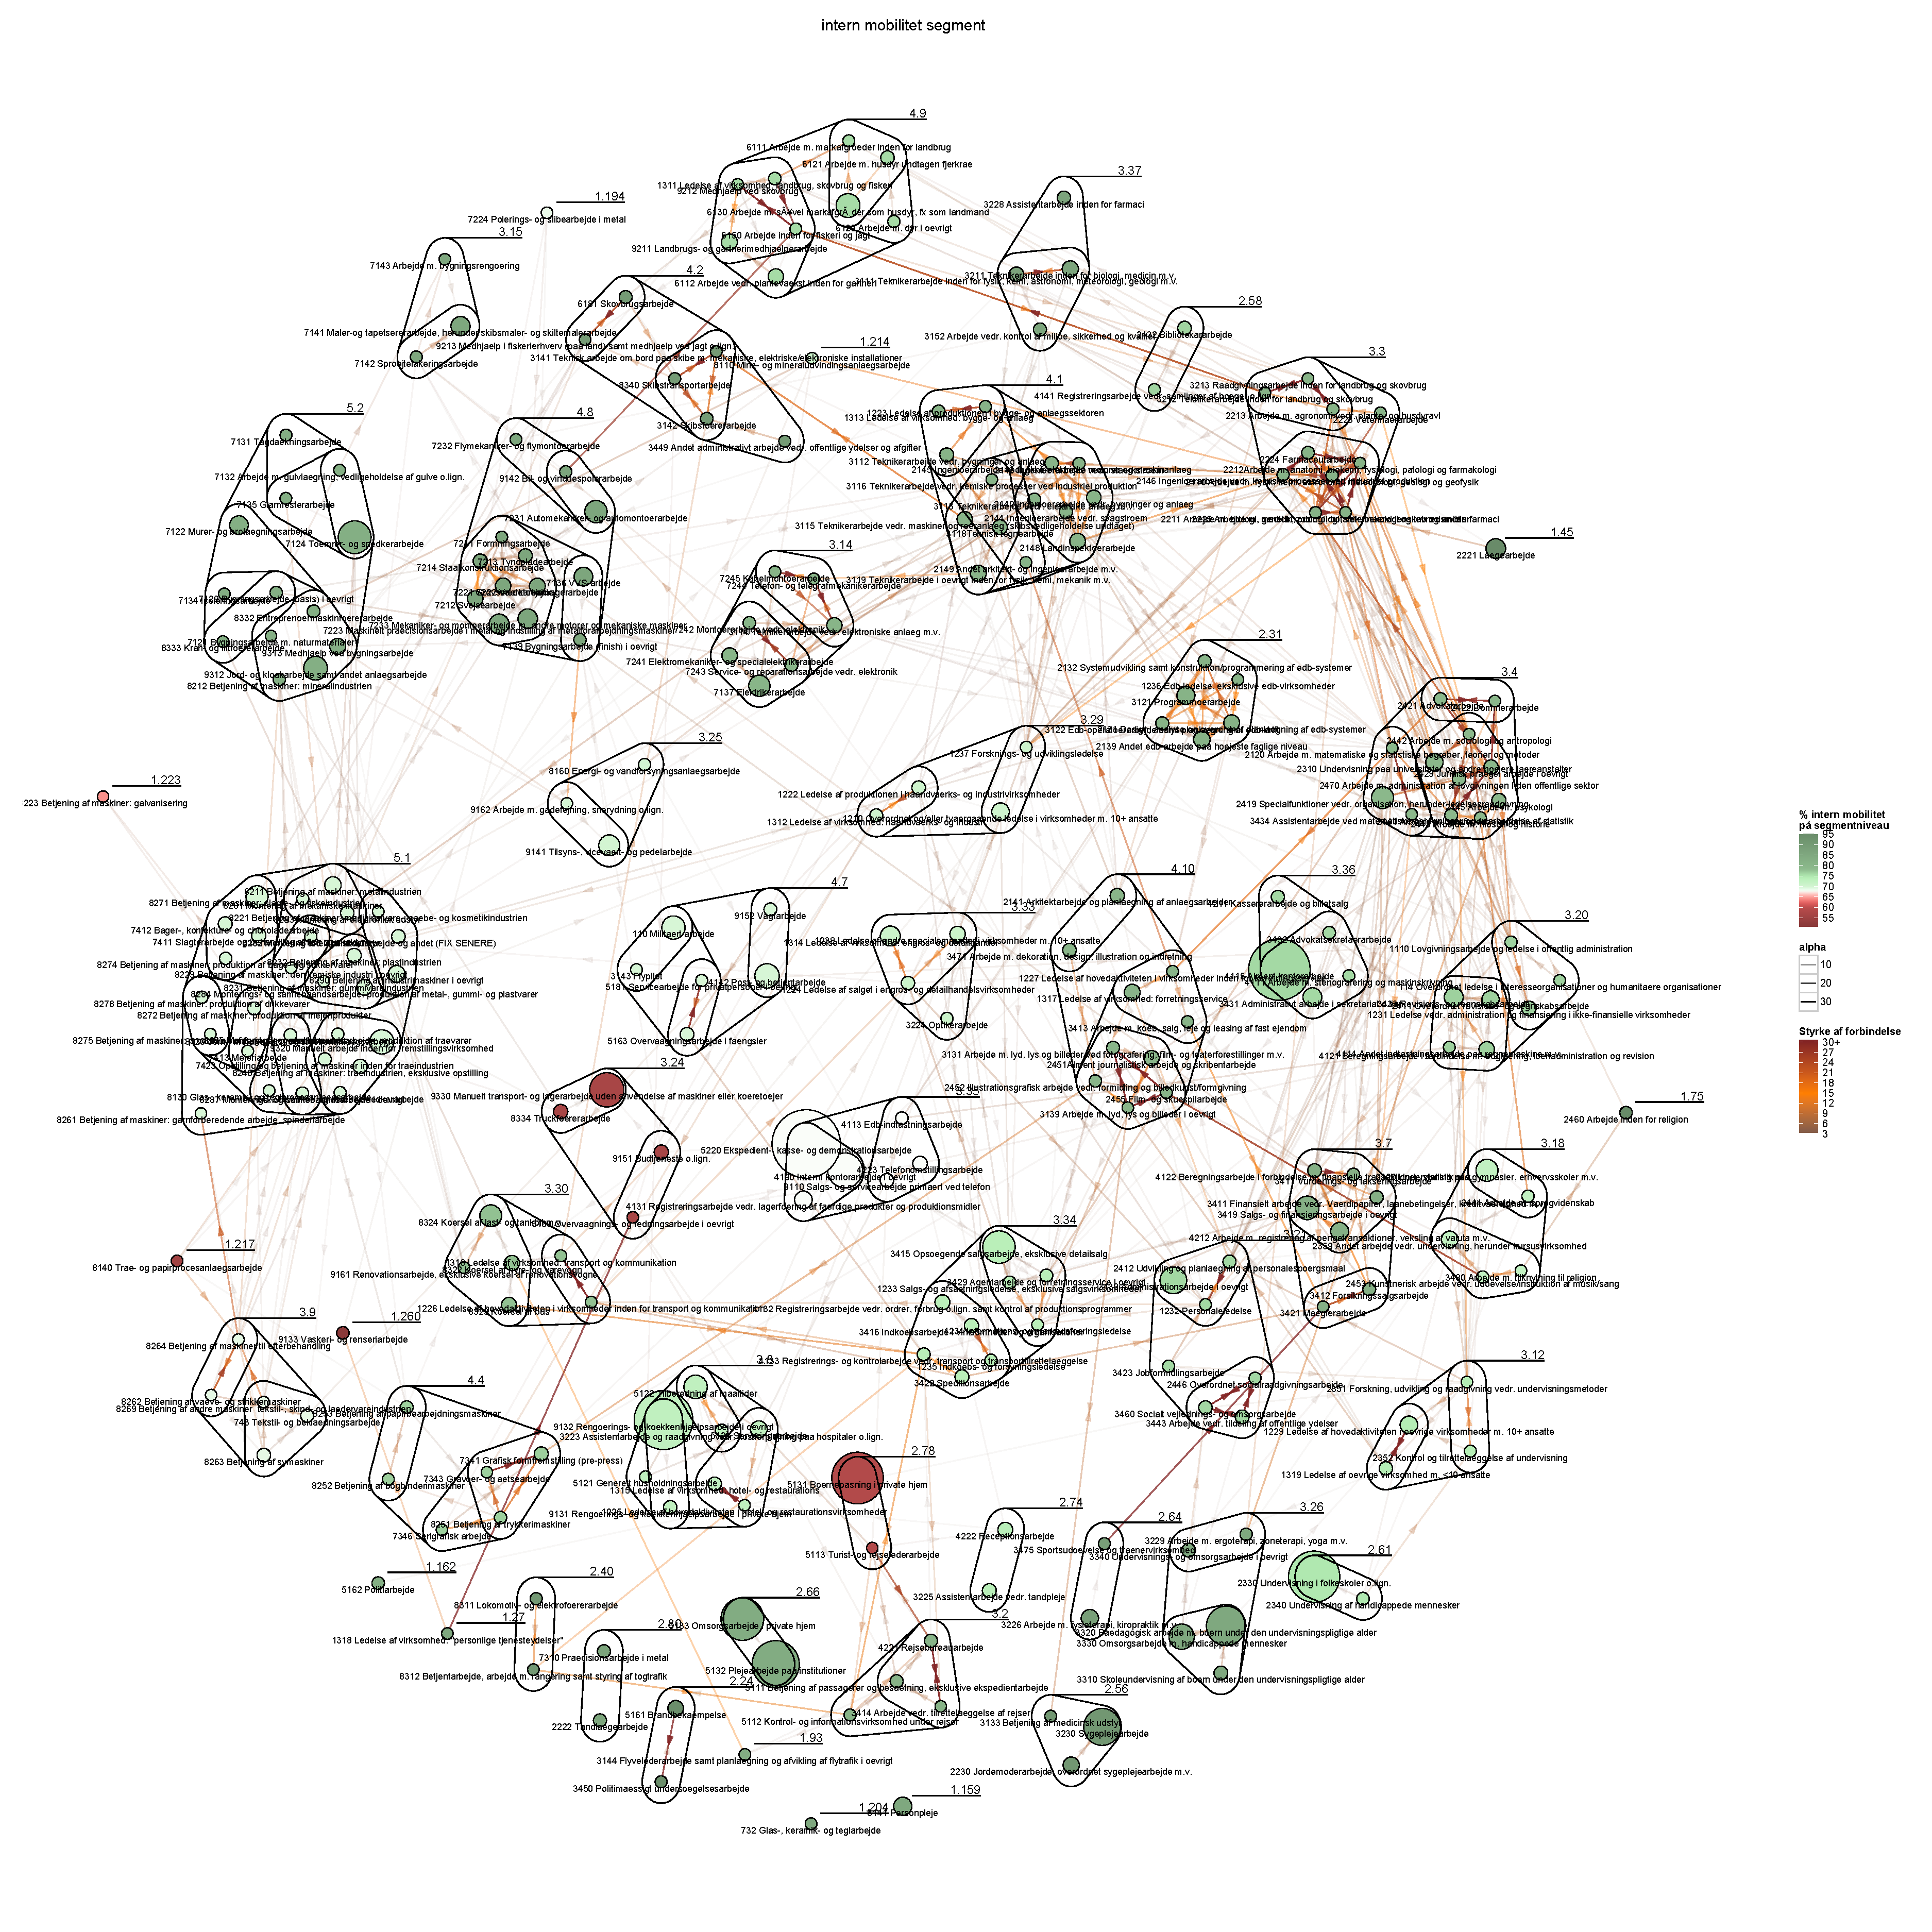
\includegraphics[width=1.0\textwidth]{fig/netvaerkskort/kort_intern_mob_seg.pdf}
\end{center}
\end{figure}
\restoregeometry
%

\underline{nodernes farve} viser andelen af den interne mobilitet indenfor klyngen. Farvespektret går fra mørkerød, til hvid, til mørkegrøn. Rød markerer en intern mobilitet på mellem 50 og 67 \%, mens hvid er medianen for den intern mobilitet, 68 \%. Grøn markerer en intern mobilitet på mellem 69 \% og 96 \%.  Da der er tale om en gradient, er skiftet i farve en kontinuer overgang, hvor intensiteten af henholdsvis rød og grøn viser hvor langt ude på skalaen vi er, i den ene eller anden retning
%
\footnote{ Skiftet i farve er, som nævnt, min egen vurdering, baseret på de deskriptive værdier for den interne mobilitet gennemgået i det foregående afsnit. Der findes ingen tidligere brug af Moneca algoritmen, hvori dette bliver analyseret, som jeg kan trække på.}%
%
. Vi kan se, at langt de fleste klynger er forskellige nuancer af grønt, hvilket viser, at langt de fleste 




\underline{forbindelsens farve} markerer som beskrevet i afsnit \ref{metode_relativrisiko} forbindelsernes styrke, målt ved den relative risiko. Et forholdsmål, læseren kan genkalde sig udtrykker mobiliteten fra en erhvervsgruppe til en anden, givet den relative størrelse af antallet af beskæftigede i erhvervsgruppen. Det er styrken af denne relative risiko (RR), der afgør farven på forbindelserne, der kan antage tre nuancer: Helt lysegrå angiver en RR på 3%
%
\footnote{Husk på den præcise definition af relativ risiko:  det vil sige, at der ved en lysegrå forbindelse er 3 gange så stor sandsynlighed for mobilitet fra den forladte beskæftigelse til den nye beskæftigelse, i forhold til hvis der var tale om et arbejdsmarked med helt fri bevægelse.}%
%
. Helt orange angiver en RR på 15. Helt mørkerød angiver en RR på 30 \emph{ eller derover}%
%
\footnote{ I bestemmelsen af klyngerne, er alle forbindelser med en RR på over 1 medtaget som en forbindelse. På det visuelle kort er den informationsmængde upraktisk. Det bliver umuligt at aflæse den underliggende systematik i hvilke forbindelser, der værd at lægge mærke til. Enkelte forbindelser har RR-værdier på flere tusinde, men de fleste langt lavere: Medianen i er på 2,1. En relativ risiko på 3 svarer cirka til den 65. percentil, og 15 er cirka den 90 percentil. 30 svarer til cirka den 92,5'te percentil, og er ikke valgt ud fra denne, men bestemt ud fra det punkt, hvor der sker en stigning i styrken af forbindelserne. }%
%
. Forbindelserne er desuden retningsbestemte, hvor pilene på kortet angiver hvilken vej, mobiliteten går.

Så vidt beskrivelsen af hvad kortet viser. Ovenstående er de generelle retningslinjer for netværkskortet: I den resterende del af analysen vil nodernes farve variere, alt efter hvilken variabel, der farvelægges efter. Fremfor at kommentere dette kort med det den interne mobilitet , vil jeg for overblikkets skyld zoome ind på nogle bestemte klynger eller delmarkeder, forklare hvad vi ser, og først derefter kommentere kortet i sin helhed.



%%%%%%%%%%%%%%%%%%%%%%%%%%%%%%%%%%%%%%%%%%%%%%
\subsection{Klynge \emak{s2.78}: Børnepasning i private hjem samt turist- og rejseledere}
%%%%%%%%%%%%%%%%%%%%%%%%%%%%%%%%%%%%%%%%%%%%%%

Hvis vi kigger på klynge \emak{s2.78}, kan vi se at den består af børnepasning i private hjem, samt turist- og rejseledere. Erhvervsgrupperne har en intern mobilitet på henholdsvis  59 \% og 47 \%, altså ganske lavt sammenlignet med den gennemsnitlige interne mobilitet på 68 \%.  Begge erhvervgrupper er indenfor hovedgruppe 5 i Disco-nomenklaturet: \texttt{salgs-, service- og omsorgsarbejde}. Det er arbejde, der ifølge Danmarks Statistik er klassificeret som ISCEDs færdighedsniveau 2, hvilket betyder at det kræver uddannelse “på grundniveau” \parencite[tabel 1]{DSTDISCO88}. Det er en klar indikator på at de formelle sociale lukningsmekanismer i disse to erhvervsgrupper er stærkt begrænsede.

%
\begin{wrapfigure}{r}{6cm}
  \vspace{-20pt}
  \begin{center}
    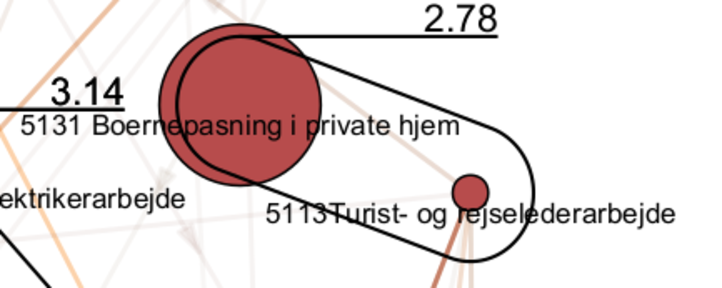
\includegraphics[width=6cm]{fig/segzoom/seg_2_78_internmob.pdf}
   \caption{}
   \label{fig_delanalyse1_zoom_2_78}
  \end{center}
  \vspace{-20pt}
\end{wrapfigure}
%

En oplagt årsag er at beskæftigelserne her simpelthen er jobs, der af den ene eller anden årsag har en karakter, der gør at folk sjældent opholder sig længe i dem. Det kunne man kalde en socialt betinget lav intern mobilitet. Hvis arbejdet har denne karakter, må man forvente, at de sociale lukningsmekanismer næppe er særlig højtudviklede. Den mest legitime af disse, i moderne samfund, må være adgangsgivende uddannelse. Vi vil derfor forvente at finde enten ufaglært fag, eller fag med lave uddannelsesmæssige krav. Det kan altså have en social årsag at den interne mobilitet er lav. Det er vigtigt at få afklaret, da disse klynger kan risikere ikke at kunne betegnes som delmarkeder i teoretisk forstand, hvis mobiliteten mellem erhvervsgrupperne ikke er hyppig. Det er ikke tegn på et metodologisk problem, men snarere et aspekt ved arbejdets karakter, og den sociale position, jobbet har på arbejdsmarkedet. I denne lille klynge er den gennemsnitlige alder 37 år%
%
\footnote{ Det også gælder de to jobs i klyngen hver især}% 
%
, hvilket er ca. 5 år under populationsgennemsnittet på 42,3 år. Vi har derfor at gøre med to erhvervsgrupper, der tiltrækker en stor andel af unge mennesker, og for hvem dette arbejde ikke nødvendigvis siger noget om hvilket delmarked, de vil indtage i deres faste klasseposition (indsæt Goldthorpe bemærkning om hvornår folk har en fast klasseposition her og find citatet \#todo). Der er naturligvis også dagplejemødre indenfor privat børnepasning, det vil sige voksne kvinder med meget tid i hjemme. Men det er rimeligt at antage at de også hopper ind og ud af andre positioner på arbejdsmarkedet. 

Hvad angår forbindelsen til turist- og rejseleder, kunne man lidt sensationsvinklet sige, at der muligvis er tale om unge, fortrinsvis piger, der passer børn som teenagere, og derefter tager til Ibiza, sydamerika eller andre steder og oplever verden. For derefter at tage sig en uddannelse.

Der er andre klynger på kortet, hvor uddannelseskravene er lave, og som befinder sig på samme færdighedsniveau indenfor ISCED-klassifikationen, men hvor den interne mobilitet alligevel er høj. Det er et sådant \underline{delmarked}, vi skal se på nu.


%%%%%%%%%%%%%%%%%%%%%%%%%%%%%%%%%%%%%%%%%%%%%%
\subsection{Delmarked \emak{s2.66}: Omsorgsarbejde i private hjem og plejearbejde på institutioner}
%%%%%%%%%%%%%%%%%%%%%%%%%%%%%%%%%%%%%%%%%%%%%%

beskæftigelsesgrupper i delmarked \emak{s2.66} befinder sig ligeledes i Discos hovedgruppe 5. Børnepasning i private hjem ligger ganske tæt på arbejdsfunktionerne i klynge \emak{s2.66}. Så tæt at de på et 3-cifret Disco niveau er kategoriseret ens, det er kun på det 4. ciffer at de adskiller sig fra hinanden. delmarked \emak{s2.66} har en intern mobilitet på 83 \%, væsentligt højere end klynge \emak{s2.78}. Det kan ikke forklares ud fra formelle inddelinger såsom Discos hovedgrupper eller ISCEDs færdighedsniveauer.

%
\begin{wrapfigure}{r}{6cm}
  \vspace{-20pt}
  \begin{center}
    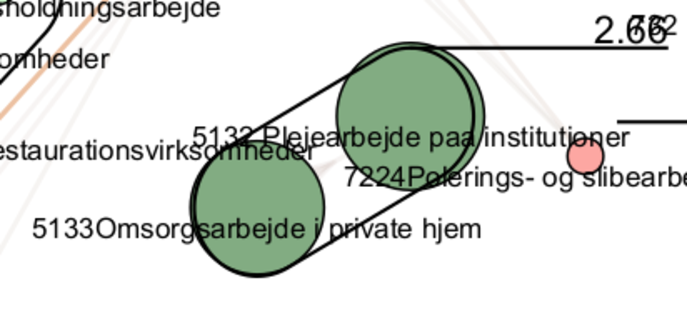
\includegraphics[width=6cm]{fig/segzoom/seg_2_66_internmob.pdf}
   \caption{}
   \label{fig_delanalyse1_zoom_2_66}
  \end{center}
  \vspace{-20pt}
\end{wrapfigure}
%

Børnepasning i private hjem har tilsyneladende en noget anden social profil. Den interne mobilitet er meget lavere, og den ligger sammen med turist- og rejseleder, der også befinder sig i hovedgruppe 5, men ikke beskæftiger sig med omsorgsarbejde for folk, der har svært ved at klare sig selv. Forskellen i social sammensætning kan aflæses i den demokrafiske sammensætning. 
%
. Delmarked \emak{s2.66} har en gennemsnitsalder på 42 $\nicefrac{3}{4}$ år, hvilket er er nærmest identisk med populationsgennemsnitet på 42,3 år. %(check hvilken kvartil det befinder sig i på forskermaskinen \#todo). 



Der er flere klynger i kortet, der viser lignende forskelle, trods samme formelle niveau i adgangskrav. Formelle færdighedsniveauer og uddannelseskrav er derfor ikke udslagsgivende for, hvorvidt der er tale om et klyng eller ej. %find eksempler \#todo


%%%%%%%%%%%%%%%%%%%%%%%%%%%%%%%%%%%%%%%%%%%%%%
\subsection{Klynge \emak{s3.24}: Transport af varer, ambulancefører og vagtarbjede}
%%%%%%%%%%%%%%%%%%%%%%%%%%%%%%%%%%%%%%%%%%%%%%

EN anden klynge \emak{s3.24} med lav intern mobilitet er en niveau 3 klynge, der indeholder to niveau 2 klynger. Den har en intern jobmobilitet på 57 \%. Der er tale om tre typer beskæftigelse, der omhandler transport af varer. Den sidste, \emak{d5169}, indeholder beskæftigelser som ambulancefører, livvagt og sikkerhedsvagt. Selvom det ikke direkte har samme omdrejningspunkt som de tre andre, fornemmer man alligevel en vis social mening i en jobcirkulation mellem de tre førnævnte, der også inkluderer denne sidste type job. 

%
\begin{wrapfigure}{r}{6cm}
  \vspace{-20pt}
  \begin{center}
    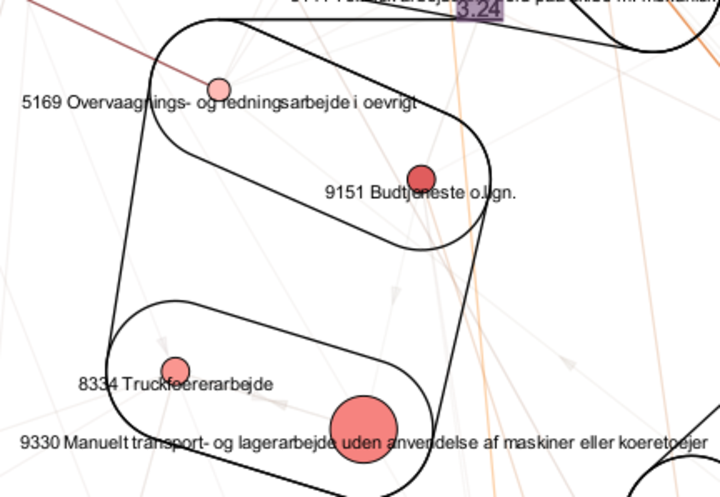
\includegraphics[width=6cm]{fig/segzoom/seg_3_24_internmob.pdf}
   \caption{}
   \label{fig_delanalyse1_zoom_3_24}
  \end{center}
  \vspace{-20pt}
\end{wrapfigure}
%

Set ud fra Goldthorpes syn på arbejdskontrakter, er det jobs, hvor specifiteten af af kompetencer er lav, og muligheden for overvågning af arbejdet må antages at være høj. Det er desuden hårdt fysisk arbejde, eller, i  tilfældet af \emak{d5169}: Arbejde, der kræver god fysisk form. Det er ikke overraskende, at denne type arbejde har en høj frafaldsprocent, da nedslidning og krav til fysik er høje. % men hvor frafalder den hen? \#todo      



%%%%%%%%%%%%%%%%%%%%%%%%%%%%%%%%%%%%%%%%%%%%%%
\section{Delkonklusion \label{}}
%%%%%%%%%%%%%%%%%%%%%%%%%%%%%%%%%%%%%%%%%%%%%%
For de fleste klynger er den interne mobilitet højere end 70 \%, det vil sige, kan karakterisers som delmarkeder. Få klynger som dem der bl.a. er blevet beskrevet ovenfå har en intern mobilitet på helt ned til 50 \%. 


Fælles for klyngerne er, at de vurderes til at være afgrænset i sådan et omfang, at der er væsentlige barrierer mellem klynget og resten af arbejdsmarkedet, der gør, at der inden for klynget er en nærhed, hvor mobilitet er “let og typisk”.

Formålet med dette kapitel har været at besvare forskningspørgsmålet: Er der en opdeling af arbejdsmarkedet for arbejdstagere i delmarkeder, hvor mobilitet indenfor delmarkederne er hyppig, og mellem delmarkederne sjælden?

Moneca-algoritmen har aggreret 273 jobfunktioner til 51 klynger. Denne opdeling afspejler Boje (1986) og Toubøl (2913). Klyngedannelsen er skabt via Moneca-algoritment og kvalitetsvurderet fra niveau til niveau. Der er i alt blevet splittet fire klynger op, som ud fra mobilitet, densitet og antal stier ikke har kunne vurderes som meningsfulde delmarkeder. 79 \% af al mobilitet foregår inden for delmarkeder, det vil sige, at mobilitet indenfor delmarkederne er hyppig, og mellem delmarkederne sjælden. Klyngerne skabt i aggreringen kan derfor betragtes som delmarkeder.



%%%%%%%%%%%%%%%%%%%%%%%%%%%%%%%%%%%%%%%%%%%%%%
% #Noter 
%%%%%%%%%%%%%%%%%%%%%%%%%%%%%%%%%%%%%%%%%%%%%%
% 
% 
%
%
%
%
%
%
%
%
%
%
%
%
%
%
%
%
% Det ses at langt de fleste klynger overholder denne beslutningsregel. 3 klynger og 3 noder ligger under 68 \%. Der er ikke er tale om en statistisk test med et vist signifikansniveau, men min egen tentative vurdering. Og selv med de vedtagne signifikansniveauer i statistiske test, eksempelvis p-værdier i en T-test eller en F-test,  der advarer litteraturen om ikke at tolke disse tærskelværdier som skrevet i sten, men som nyttige konventioner (find henvisning, Gujarati og Malchow-Møller \#todo) (blah blah).